\documentclass[a4paper,12pt,oneside]{report}
% ======================================================================
%  Định dạng báo cáo — theo mẫu Tiểu luận 03 (Times 13pt, giãn dòng 1.5)
% ======================================================================
\usepackage[a4paper,left=3cm,right=2cm,top=2.5cm,bottom=2.5cm,headheight=14pt]{geometry}
\usepackage{fontspec}
\usepackage{unicode-math}
\setmainfont{TeX Gyre Termes}[Scale=1.0833]          % 12pt × 1,0833 ≈ 13pt
\setmathfont{TeX Gyre Termes Math}[Scale=1.0833]
\setmonofont{SourceCodePro}[Extension=.otf,UprightFont=*-Regular,BoldFont=*-Bold,ItalicFont=*-RegularIt,BoldItalicFont=*-BoldIt,Scale=0.82]
\usepackage{polyglossia}
\setdefaultlanguage{vietnamese}
\setotherlanguage{english}  % để biblatex dùng chuỗi tiếng Anh (đã Việt hóa) trong danh mục tài liệu

\usepackage{setspace}
\setstretch{1.4}
\setlength{\parindent}{1cm}
\setlength{\parskip}{3pt}
\usepackage{indentfirst}
\usepackage{microtype}
\usepackage{ragged2e}
\setlength{\emergencystretch}{3em}

\usepackage{amsmath,amsthm}
\usepackage{graphicx}
\graphicspath{{figures/}}
\usepackage{float}
\usepackage{booktabs,longtable,tabularx,multirow,array,makecell}
\renewcommand{\arraystretch}{1.18}
\usepackage{xcolor}
\definecolor{codebg}{HTML}{F4F5F7}
\definecolor{accent}{HTML}{1D4ED8}
\usepackage[hidelinks]{hyperref}
\usepackage{xurl}
\usepackage[htt]{hyphenat}  % cho phép ngắt dòng trong \texttt (tên hàm, đường dẫn dài)
\usepackage{adjustbox}
\usepackage{enumitem}
\setlist{itemsep=1pt,topsep=3pt,parsep=0pt,leftmargin=1.2cm}
\usepackage{tikz}
\usetikzlibrary{positioning,arrows.meta,shapes.geometric,shapes.symbols,calc,fit,backgrounds}

% ---------------------------------------------------------------- tiêu đề chương, mục
\usepackage{titlesec}
\titleformat{\chapter}[block]{\centering\bfseries\fontsize{15}{19}\selectfont}
  {\MakeUppercase{\chaptertitlename}\ \thechapter.}{0.5em}{\MakeUppercase}
\titlespacing{\chapter}{0pt}{-10pt}{18pt}
\titleformat{\section}{\bfseries\fontsize{13.5}{17}\selectfont}{\thesection.}{0.5em}{}
\titleformat{\subsection}{\bfseries\itshape\fontsize{13}{16}\selectfont}{\thesubsection.}{0.5em}{}
\titleformat{\subsubsection}{\itshape\fontsize{13}{16}\selectfont}{\thesubsubsection.}{0.5em}{}
\titlespacing{\section}{0pt}{10pt}{4pt}
\titlespacing{\subsection}{0pt}{8pt}{3pt}
\titlespacing{\subsubsection}{0pt}{6pt}{2pt}
\setcounter{secnumdepth}{3}
\setcounter{tocdepth}{2}
\renewcommand{\chaptertitlename}{Chương}

% chương không đánh số (Mở đầu, Kết luận, TLTK) vẫn vào mục lục
\newcommand{\unnumberedchapter}[1]{%
  \chapter*{#1}\addcontentsline{toc}{chapter}{#1}\markboth{#1}{#1}}

% ---------------------------------------------------------------- mục lục
\usepackage{tocloft}
\renewcommand{\contentsname}{\centering MỤC LỤC}
\renewcommand{\listfigurename}{\centering DANH MỤC HÌNH VẼ}
\renewcommand{\listtablename}{\centering DANH MỤC BẢNG BIỂU}
\renewcommand{\cftchapfont}{\bfseries}
\renewcommand{\cftchappagefont}{\bfseries}
\renewcommand{\cftchappresnum}{CHƯƠNG }
\setlength{\cftchapnumwidth}{6.6em}
\renewcommand{\cftchapaftersnum}{.}
\renewcommand{\cftsecaftersnum}{.}
\renewcommand{\cftsubsecaftersnum}{.}
\renewcommand{\cftchapleader}{\cftdotfill{\cftdotsep}}
\renewcommand{\cftfigpresnum}{Hình }
\renewcommand{\cfttabpresnum}{Bảng }
\setlength{\cftfignumwidth}{5.2em}
\setlength{\cfttabnumwidth}{5.2em}
\renewcommand{\cftfigaftersnum}{.}
\renewcommand{\cfttabaftersnum}{.}

% ---------------------------------------------------------------- chú thích hình, bảng
\usepackage{caption}
\DeclareCaptionLabelSeparator{dotspace}{.\ }
\captionsetup{labelsep=dotspace,font={small},justification=centering,singlelinecheck=false}
\captionsetup[figure]{name=Hình,font={small,it},skip=4pt}
\captionsetup[table]{name=Bảng,font={small,bf},position=top,skip=4pt}
\renewcommand{\thefigure}{\thechapter.\arabic{figure}}
\renewcommand{\thetable}{\thechapter.\arabic{table}}

% ---------------------------------------------------------------- đoạn mã
\usepackage[newfloat]{minted}
\setminted{fontsize=\footnotesize,breaklines,bgcolor=codebg,frame=none,tabsize=4,
           baselinestretch=1.05,style=friendly,autogobble}
\SetupFloatingEnvironment{listing}{name=Đoạn mã,placement=H}
\captionsetup[listing]{font={small,bf},position=top,justification=raggedright,skip=2pt}
\renewcommand{\thelisting}{\thechapter.\arabic{listing}}
\newenvironment{code}[1]{\begin{listing}[H]\caption{#1}}{\end{listing}}

% ---------------------------------------------------------------- trang
\usepackage{fancyhdr}
\pagestyle{fancy}
\fancyhf{}
\fancyfoot[C]{\thepage}
\renewcommand{\headrulewidth}{0pt}
\fancypagestyle{plain}{\fancyhf{}\fancyfoot[C]{\thepage}\renewcommand{\headrulewidth}{0pt}}

% ---------------------------------------------------------------- tài liệu tham khảo
\usepackage[backend=biber,style=ieee,sorting=none,maxnames=4,minnames=1,language=english,autolang=none]{biblatex}
\addbibresource{refs.bib}
\DefineBibliographyStrings{english}{andothers={và cộng sự},and={và},in={trong},edition={ấn bản},volume={tập},jourvol={tập},number={số},pages={tr.},page={tr.}}

% ---------------------------------------------------------------- tiện ích
\newcommand{\eq}[1]{(\ref{#1})}
\newcommand{\figref}[1]{Hình~\ref{#1}}
\newcommand{\tabref}[1]{Bảng~\ref{#1}}
\newcommand{\coderef}[1]{Đoạn mã~\ref{#1}}
\newcommand{\weburl}[1]{{\small\url{#1}}}
\newcommand{\api}[1]{\texttt{\small #1}}
\newcommand{\figw}[3][\linewidth]{%
  \begin{figure}[H]\centering\includegraphics[width=#1]{#2}\caption{#3}\label{fig:#2}\end{figure}}
\newcolumntype{L}[1]{>{\raggedright\arraybackslash}p{#1}}
\newcolumntype{C}[1]{>{\centering\arraybackslash}p{#1}}
\newcolumntype{Y}{>{\raggedright\arraybackslash}X}
\newtheorem*{dinhnghia}{Định nghĩa}

% tên miền triển khai (Cloudflare Tunnel) — đổi ở đây là đổi toàn bộ báo cáo
\newcommand{\deploydomain}{agent.nits.io.vn}
\newcommand{\agent}[1]{\texttt{#1}}


\begin{document}

% ====================================================================== BÌA (cùng mẫu với tiểu luận final)
\pagenumbering{Alph}
\begin{titlepage}
\begin{tikzpicture}[remember picture,overlay]
  \draw[line width=1.6pt] ($(current page.north west)+(2.3cm,-1.8cm)$) rectangle ($(current page.south east)+(-1.5cm,1.8cm)$);
  \draw[line width=0.5pt] ($(current page.north west)+(2.45cm,-1.95cm)$) rectangle ($(current page.south east)+(-1.65cm,1.95cm)$);
\end{tikzpicture}
\centering
\setstretch{1.25}
\vspace*{0.4cm}
{\bfseries HỌC VIỆN CÔNG NGHỆ BƯU CHÍNH VIỄN THÔNG\\[2pt] KHOA CÔNG NGHỆ THÔNG TIN 1\\[-4pt]}
\rule{5.2cm}{0.5pt}

\vspace{1.0cm}

\includegraphics[height=3.4cm]{ptit_logo}

\vspace{1.0cm}
{\fontsize{19}{25}\selectfont\bfseries PROJECT 01\\[4pt] PHÁT TRIỂN HỆ THỐNG THÔNG MINH\par}
\vspace{1.1cm}
{\fontsize{14.5}{20}\selectfont\bfseries HỆ ĐA AGENT CHO BỆNH TIỂU ĐƯỜNG\par}
\vspace{0.4cm}
{\itshape Deep Learning, Knowledge Base (Neo4j) và RAG,\\ Reinforcement Learning kết hợp luật, hội đồng tranh biện\par}

\vspace{1.6cm}
\begin{tabular}{@{}l@{\hspace{1.2cm}}l@{}}
\textbf{Giảng viên hướng dẫn:} & PGS. TS. Trần Đình Quế \\
\textbf{Sinh viên thực hiện:} & Nguyễn Tự Kiên \\
\textbf{Mã sinh viên:} & B23DCCN465 \\
\textbf{Nhóm lớp:} & CT01 \\
\textbf{Nhóm:} & 07 \\
\end{tabular}

\vfill
{\bfseries Hà Nội, tháng 11 năm 2026\par}
\vspace{0.6cm}
\end{titlepage}

% ====================================================================== PHẦN ĐẦU
\pagenumbering{roman}
\setcounter{page}{2}
\begin{spacing}{1.15}
\tableofcontents
\end{spacing}
\clearpage
\chapter*{DANH MỤC TỪ VIẾT TẮT}
\addcontentsline{toc}{chapter}{DANH MỤC TỪ VIẾT TẮT}
\begin{spacing}{1.1}
\small
\begin{longtable}{@{}L{2.3cm}L{6.3cm}L{6.0cm}@{}}
\toprule
\textbf{Viết tắt} & \textbf{Tiếng Anh} & \textbf{Tiếng Việt} \\
\midrule
\endhead
ADA & American Diabetes Association & Hiệp hội Đái tháo đường Hoa Kỳ \\
AUC & Area Under the (ROC) Curve & Diện tích dưới đường ROC \\
BM25 & Best Matching 25 & Hàm xếp hạng BM25 \\
BMI & Body Mass Index & Chỉ số khối cơ thể \\
DL & Deep Learning & Học sâu \\
ĐTĐ & -- & Đái tháo đường \\
FIPA-ACL & FIPA Agent Communication Language & Ngôn ngữ giao tiếp tác tử FIPA \\
FPG & Fasting Plasma Glucose & Glucose huyết tương lúc đói \\
FTS & Full-Text Search & Tìm kiếm toàn văn \\
GBDT & Gradient Boosted Decision Trees & Cây quyết định tăng cường gradient \\
HbA1c & Glycated Hemoglobin & Huyết sắc tố gắn glucose \\
HNSW & Hierarchical Navigable Small World & Đồ thị thế giới nhỏ phân cấp \\
KB & Knowledge Base & Cơ sở tri thức \\
KG & Knowledge Graph & Đồ thị tri thức \\
LLM & Large Language Model & Mô hình ngôn ngữ lớn \\
MAS & Multi-Agent System & Hệ đa tác tử (hệ đa agent) \\
MDP & Markov Decision Process & Quá trình quyết định Markov \\
ML & Machine Learning & Học máy \\
MLP & Multilayer Perceptron & Mạng nơ-ron nhiều lớp \\
NHANES & National Health and Nutrition Examination Survey & Khảo sát Sức khỏe và Dinh dưỡng Quốc gia Hoa Kỳ \\
OGTT & Oral Glucose Tolerance Test & Nghiệm pháp dung nạp glucose đường uống \\
RAG & Retrieval-Augmented Generation & Sinh văn bản tăng cường truy xuất \\
RL & Reinforcement Learning & Học tăng cường \\
RRF & Reciprocal Rank Fusion & Gộp xếp hạng nghịch đảo \\
\bottomrule
\end{longtable}
\end{spacing}

\clearpage
\begin{spacing}{1.1}
\listoffigures
\clearpage
\listoftables
\end{spacing}
\clearpage

% ====================================================================== NỘI DUNG (theo dàn ý trên bảng)
\pagenumbering{arabic}
\chapter{Giới thiệu}
\label{chap:intro}

\section{Bài toán và động lực}

Đái tháo đường (ĐTĐ, bệnh tiểu đường) là tình trạng glucose trong máu tăng cao kéo dài do cơ thể thiếu insulin hoặc kháng insulin. Phần lớn ca bệnh là ĐTĐ típ 2, loại tiến triển âm thầm nhiều năm và có thể làm chậm hoặc phòng ngừa nếu phát hiện sớm từ giai đoạn tiền ĐTĐ \cite{ada2024,knowler2002dpp}. Ở Việt Nam, Hướng dẫn chẩn đoán và điều trị ĐTĐ típ 2 của Bộ Y tế \cite{byt5481} khuyến cáo sàng lọc chủ động cho người có yếu tố nguy cơ, nhưng người dân thường chỉ có trong tay vài con số rời rạc (một lần thử đường huyết, cân nặng, huyết áp) và không biết chúng nói lên điều gì.

Một công cụ hỗ trợ sàng lọc tốt phải làm được bốn việc cùng lúc: \emph{dự đoán} nguy cơ từ dữ liệu sức khỏe; \emph{giải thích} dựa trên tri thức y khoa có nguồn; \emph{gợi ý} bước can thiệp cụ thể; và \emph{cảnh báo} ngay khi có dấu hiệu nguy hiểm. Mỗi việc cần một kỹ thuật khác nhau: học sâu cho dự đoán, cơ sở tri thức và RAG cho giải thích, học tăng cường cho ra quyết định tuần tự, và luật cố định cho an toàn. Gộp tất cả vào một chương trình khiến hệ thống khó kiểm tra và khó tin cậy. Vì vậy project xây dựng một \textbf{hệ đa agent}: mỗi agent giữ một chuyên môn, các agent trao đổi bằng thông điệp có cấu trúc, và một hội đồng kiểm tra chéo kết luận trước khi tư vấn cho người dùng.

\section{Mục tiêu và phạm vi}

Project hiện thực hóa sơ đồ mà giảng viên đưa ra trên lớp (\figref{fig:board}, Chương~\ref{chap:arch}) thành một hệ thống chạy được đầu–cuối:
\begin{itemize}
  \item \textbf{DB → Deep Learning → dự đoán, phân loại}: huấn luyện mô hình học máy và mạng nơ-ron trên hai bộ dữ liệu có sẵn của CDC, tổng cộng \textbf{3.193.465 người}: NHANES 2011–2018 (20.646 người, nhãn xác nhận bằng xét nghiệm) làm mô hình chính, và BRFSS 2011–2023 (\textbf{3.172.819 người}, bảy năm khảo sát) làm mô hình quy mô lớn; ước lượng xác suất ĐTĐ rồi phân tầng nguy cơ thành bốn mức.
  \item \textbf{Web, sách → Neo4j KB → RAG}: nạp hướng dẫn ADA 2024 và QĐ 5481/QĐ-BYT vào cơ sở tri thức; đồ thị tri thức lưu trên \textbf{Neo4j}, đoạn văn được tìm kiếm lai trên \textbf{Qdrant} (vector) và \textbf{SQLite FTS5} (toàn văn).
  \item \textbf{Reinforcement learning + rule → Agent}: agent gợi ý can thiệp học bằng Q-learning nhưng bị ràng buộc bởi luật an toàn và kết luận của hội đồng.
  \item \textbf{Tư vấn, trợ giúp}: hội đồng tranh biện liệt kê bằng chứng đồng thuận (+) và mâu thuẫn (−), rồi agent phản hồi viết câu trả lời có trích dẫn.
  \item \textbf{Code + Demo}: chatbot web kèm \emph{Phòng hội chẩn} trực quan hóa từng thông điệp giữa các agent; mã nguồn có kiểm thử tự động.
\end{itemize}

\textbf{Phạm vi.} Đây là sản phẩm học tập. Hệ thống phục vụ \emph{sàng lọc} chứ không \emph{chẩn đoán}, không đưa liều thuốc cụ thể, và mọi câu trả lời đều nhắc người dùng đi khám bác sĩ. Mọi con số trong báo cáo được đo lại từ mã nguồn của project.

\section{Đóng góp và cấu trúc báo cáo}

Các đóng góp chính:
\begin{itemize}
  \item Một hệ \textbf{chín agent} giao tiếp qua \texttt{MessageBus} theo tinh thần FIPA-ACL, có audit trail đầy đủ và cô lập lỗi.
  \item Khối DB gồm \textbf{hơn 3,19 triệu hồ sơ} thật của CDC, gấp hơn 12 lần bản BRFSS 2015 đã làm sạch (253.680 dòng) thường được dùng cho bài toán này. Mô hình huấn luyện trên dữ liệu quy mô lớn đóng vai \emph{ý kiến thứ hai}, và hội đồng chất vấn khi nó ngược với mô hình chính.
  \item Hai nhánh song song đúng như sơ đồ: \emph{DB → ML/DL} và \emph{KB (Neo4j) → RAG}, gặp nhau ở một hội đồng có \textbf{tranh biện nhiều vòng}: agent phản biện chất vấn agent chuyên môn khi chúng mâu thuẫn.
  \item Agent \textbf{RL + luật}: chính sách Q-learning chỉ được hành động trong khuôn khổ do tri thức tường minh cho phép.
  \item \textbf{Phòng hội chẩn}: giao diện phát lại luồng thông điệp, cho người xem thấy agent nào đang nói gì với agent nào.
  \item Đánh giá trên 634.564 hồ sơ BRFSS kiểm tra và đánh giá đầu–cuối trên 400 ca NHANES chưa từng thấy; đo lại truy xuất RAG trên bộ lưu trữ mới.
\end{itemize}

Báo cáo đi theo đúng dàn ý trên bảng. Chương~\ref{chap:mas} trình bày cơ sở về agent và hệ đa agent. Chương~\ref{chap:arch} là kiến trúc tổng quan. Chương~\ref{chap:comp} mô tả từng thành phần: Deep Learning, KB và RAG, RL kết hợp luật, hội đồng và tầng tiếp nhận. Chương~\ref{chap:code} trình bày mã nguồn, demo, kiểm thử và đánh giá. Cuối cùng là kết luận.

\chapter{Hệ đa agent}
\label{chap:mas}

\section{Agent}

Theo Wooldridge \cite{wooldridge2009}, \emph{agent} (tác tử) là một hệ thống tính toán đặt trong một môi trường, có khả năng \emph{hành động tự chủ} trong môi trường đó để đạt mục tiêu được giao. Điều cốt lõi là vòng lặp \emph{quan sát → quyết định → hành động → nhận phản hồi}, chứ không chỉ là một hàm trả về kết quả. Một agent thông minh có bốn tính chất \cite{jennings1998}:
\begin{itemize}
  \item \textbf{Tự chủ}: tự quyết định hành động mà không cần con người can thiệp từng bước.
  \item \textbf{Phản ứng}: nhận biết thay đổi của môi trường và phản hồi kịp thời.
  \item \textbf{Chủ động}: hướng tới mục tiêu, tự khởi xướng hành động.
  \item \textbf{Xã hội}: tương tác với agent khác và với con người qua một ngôn ngữ giao tiếp.
\end{itemize}

\begin{figure}[H]
\centering
\begin{tikzpicture}[font=\small,
  box/.style={draw, rounded corners=3pt, align=center, minimum height=10mm, text width=3.2cm, inner sep=3pt},
  arr/.style={-{Stealth[length=2mm]}, thick, black!60}]
\node[box, fill=blue!6] (agent) at (0,0) {\textbf{Agent}\\ chương trình + trạng thái};
\node[box, fill=gray!10] (env) at (7,0) {\textbf{Môi trường}\\ người dùng, hồ sơ, agent khác};
\draw[arr] (env.north west) to[bend right=25] node[above]{quan sát (thông điệp, dữ liệu)} (agent.north east);
\draw[arr] (agent.south east) to[bend right=25] node[below]{hành động (trả lời, chất vấn, đề xuất)} (env.south west);
\end{tikzpicture}
\caption{Vòng lặp quan sát – hành động của một agent}
\label{fig:agent-loop}
\end{figure}

Russell và Norvig \cite{russell2021} phân loại agent theo độ phức tạp của chương trình bên trong. \tabref{tab:agent-types} đặt các agent của project vào cách phân loại đó: mỗi loại đều có mặt trong hệ thống.

\begin{table}[H]
\centering
\caption{Các loại agent và hiện thực trong project}
\label{tab:agent-types}
\small
\begin{tabularx}{\linewidth}{@{}L{3.6cm}L{4.4cm}Y@{}}
\toprule
\textbf{Loại agent} & \textbf{Cách ra quyết định} & \textbf{Trong project} \\
\midrule
Phản xạ theo luật & Nếu điều kiện thì hành động; không học & Safety Guardrail trong \agent{ConsensusCriticAgent}, \agent{ClarificationAgent} (luật phạm vi) \\
Phản xạ có mô hình & Duy trì trạng thái nội tại & \agent{ConversationAgent}, \agent{DocumentAgent} cập nhật hồ sơ \texttt{PatientProfile} \\
Dựa trên mục tiêu & Lập kế hoạch để đạt mục tiêu & \agent{Orchestrator} lập kế hoạch động cho từng lượt chat \\
Dựa trên tri thức & Suy luận trên tri thức tường minh & \agent{KnowledgeAgent}: ngưỡng ADA, đồ thị Neo4j, RAG \\
Agent học & Cải thiện từ dữ liệu, phần thưởng & \agent{PredictionAgent} (GBDT + MLP), \agent{TreatmentRLAgent} (Q-learning) \\
\bottomrule
\end{tabularx}
\end{table}

\section{Hệ đa agent}

Hệ đa agent (Multi-Agent System, MAS) gồm nhiều agent tương tác để giải quyết bài toán vượt quá khả năng hoặc hiểu biết của từng agent. Nếu chỉ có một agent làm tất cả, nó phải trộn dữ liệu số, văn bản y khoa, chính sách can thiệp và luật an toàn trong cùng một chỗ: khó kiểm thử, khó thay thế, và khó biết kết luận đến từ đâu. \tabref{tab:single-vs-mas} so sánh hai cách làm.

\begin{table}[H]
\centering
\caption{Một agent làm tất cả so với hệ đa agent của project}
\label{tab:single-vs-mas}
\small
\begin{tabularx}{\linewidth}{@{}L{3.4cm}YY@{}}
\toprule
\textbf{Tiêu chí} & \textbf{Một agent} & \textbf{Hệ đa agent (project)} \\
\midrule
Độ phức tạp mỗi phần & Cao, trộn nhiều kỹ thuật & Thấp, mỗi agent một kỹ thuật \\
Kiểm thử & Khó tách lỗi & Kiểm thử từng agent và cả hội đồng (43 test tự động) \\
An toàn & Luật nằm lẫn trong mô hình & Guardrail độc lập, luôn được ưu tiên \\
Kiểm tra chéo & Không có & Hội đồng chất vấn khi các agent mâu thuẫn \\
Chịu lỗi & Một lỗi làm hỏng cả lượt & Lỗi của một agent thành thông điệp \texttt{FAILURE} \\
Chi phí phối hợp & Không có & Cần điều phối và giao thức thông điệp \\
\bottomrule
\end{tabularx}
\end{table}

\textbf{Mô hình tổ chức.} Các kiểu tổ chức MAS phổ biến gồm: \emph{Supervisor} (một agent điều phối giao việc và tổng hợp kết quả); \emph{Blackboard} \cite{hayesroth1985} (các agent đọc ghi một vùng nhớ dùng chung); \emph{Contract Net} \cite{smith1980} (giao việc qua đấu thầu); và \emph{tranh biện ngang hàng}, nơi các agent trao đổi lập luận tới khi đồng thuận \cite{du2024debate}. Project kết hợp ba kiểu: \agent{Orchestrator} là supervisor; hồ sơ bệnh nhân \texttt{PatientProfile} là blackboard tích lũy qua nhiều lượt chat; và \agent{ConsensusCriticAgent} điều khiển tranh biện giữa các agent chuyên môn.

\section{Giao tiếp giữa các agent}

FIPA-ACL \cite{fipa2002} chuẩn hóa thông điệp giữa các agent: mỗi thông điệp có người gửi, người nhận, nội dung, và một \emph{performative} thể hiện ý định giao tiếp. Performative tách ``nói gì'' khỏi ``muốn gì'', nên agent nhận biết cần thực hiện, trả lời hay chỉ ghi nhận. Project dùng năm performative:

\begin{table}[H]
\centering
\caption{Năm performative dùng trong hệ thống}
\label{tab:perf}
\small
\begin{tabularx}{\linewidth}{@{}L{2.6cm}Y L{4.6cm}@{}}
\toprule
\textbf{Performative} & \textbf{Ý nghĩa} & \textbf{Ví dụ} \\
\midrule
\texttt{REQUEST} & Yêu cầu agent khác thực hiện một việc & Orchestrator → Prediction: \texttt{PREDICT\_RISK} \\
\texttt{INFORM} & Trả kết quả của việc được giao & Prediction → Orchestrator: \texttt{RISK\_PREDICTION} \\
\texttt{CHALLENGE} & Chất vấn khi phát hiện mâu thuẫn & Critic → Prediction: \texttt{CHALLENGE\_ML\_VS\_LABS} \\
\texttt{RESPONSE} & Trả lời chất vấn: bảo vệ, nhượng bộ hoặc giải trình & Prediction → Critic: giữ quan điểm ``nguy cơ dài hạn'' \\
\texttt{FAILURE} & Không thực hiện được (lỗi, không hiểu yêu cầu) & \texttt{NOT\_UNDERSTOOD}, \texttt{PREDICT\_RISK\_FAILED} \\
\bottomrule
\end{tabularx}
\end{table}

Từ 2023, mô hình ngôn ngữ lớn (LLM) thường được dùng làm ``bộ não'' của agent, như ReAct \cite{yao2023react}, AutoGen \cite{wu2023autogen} hay MetaGPT \cite{hong2024metagpt}. Các khảo sát \cite{wang2024agents,guo2024mas} chỉ ra ba thách thức: ảo giác lan truyền giữa các agent, chi phí của nhiều lần gọi LLM, và khó kiểm soát khi agent tự quyết định luồng. Project chọn hướng \emph{lai}: LLM chỉ hiểu và diễn đạt ngôn ngữ (trích chỉ số từ tin nhắn, đọc ảnh, viết câu trả lời), còn mọi quyết định lâm sàng do mô hình đã đánh giá và luật tường minh đảm nhận. Nhờ vậy hệ thống chạy được hoàn toàn \emph{không cần LLM}, kết quả tái lập được.

\chapter{Kiến trúc tổng quan}
\label{chap:arch}

\section{Sơ đồ của đề bài và hiện thực}

\figref{fig:board} vẽ lại sơ đồ trên bảng, giữ nguyên bố cục, và ghi kèm (chữ nghiêng màu xám) thành phần hiện thực tương ứng trong project. Có ba dòng chảy hội tụ vào agent trung tâm: (1) dữ liệu \emph{có sẵn} đi qua Deep Learning để \emph{dự đoán} và \emph{phân loại}; (2) tri thức từ web, sách được \emph{tạo} thành Knowledge Base trên Neo4j và truy xuất bằng RAG; (3) reinforcement learning và luật (rule) cùng điều khiển agent ra quyết định. Kết quả hội tụ ở vòng tròn lớn: hội đồng \emph{tư vấn} và \emph{trợ giúp} người dùng.

\begin{figure}[H]
\centering
\begin{tikzpicture}[font=\small,
  box/.style={draw, thick, align=center, minimum height=8mm, inner sep=4pt},
  note/.style={font=\scriptsize\itshape, text=black!55, align=center},
  arr/.style={-{Stealth[length=2.2mm]}, thick}]
% --- hàng 1: DB → Deep learning → dự đoán / phân loại
\node[draw, thick, cylinder, shape border rotate=90, aspect=0.25, minimum width=2.1cm, minimum height=1.5cm, align=center] (db) at (0,0) {DB};
\node[note, below=1mm of db] (dbn) {có sẵn (SQLite): NHANES 20.646 người\\ + BRFSS 2011–2023: 3.172.819 người};
\node[box] (dl) at (4.3,1.35) {Deep learning};
\node[note, above=0.5mm of dl] {GBDT + MLP (PyTorch), 2 bộ dữ liệu};
\coordinate (mid) at (4.3,0);
\draw[arr] (db.east) -- (5.6,0);
\draw[arr, dashed] (dl.south) -- (mid);
\node[box, anchor=west] (pred) at (6.6,0.55) {Dự đoán};
\node[box, anchor=west] (cls) at (6.6,-0.55) {Phân loại};
\draw[thick] (5.6,0) -- (6.1,0); \draw[thick] (6.1,0.55) -- (6.1,-0.55);
\draw[arr] (6.1,0.55) -- (pred.west); \draw[arr] (6.1,-0.55) -- (cls.west);
\node[note, right=1mm of pred] {xác suất ĐTĐ};
\node[note, right=1mm of cls] {4 mức nguy cơ};

% --- hàng 2: neo4j KB + RAG → Agent
\node[box, minimum width=2.1cm] (neo) at (0,-3.0) {neo4j};
\node[box, minimum width=2.1cm, below=0pt of neo, font=\bfseries\large] (kb) {KB};
\node[note, left=1mm of kb, text width=2.2cm] {34 nút, 40 cạnh\\ + 36 đoạn văn};
\node[draw, thick, cloud, cloud puffs=11, aspect=2, align=center, inner sep=0pt] (web) at (-0.4,-5.6) {web, book};
\node[note, below=0.5mm of web] {ADA 2024 · QĐ 5481/QĐ-BYT};
\draw[arr] (web.north) -- node[left, font=\scriptsize]{tạo} (kb.south -| web.north);
\node[box] (rag) at (4.3,-2.6) {RAG};
\node[note, right=1mm of rag, text width=2.6cm] {Qdrant (vector) + FTS5 (toàn văn) + GraphRAG};
\node[box, minimum width=1.9cm] (agent) at (4.3,-4.5) {Agent};
\node[note, right=1mm of agent, text width=2.4cm] {9 agent qua MessageBus};
\draw[thick] (kb.east |- 0,-3.55) -- node[above, font=\large]{+} (3.3,-3.55);
\draw[thick] (3.3,-3.55) -- (8.3,-3.55);
\draw[thick] (rag.south) -- (4.3,-3.55); \draw[thick] (4.3,-3.55) -- (agent.north);

% --- hàng 3: reinforcement learning + rule → Agent
\node[box, text width=2.5cm] (rl) at (3.2,-6.7) {reinforcement learning};
\node[box] (rule) at (6.3,-6.7) {rule};
\node[note, below=0.5mm of rl, text width=3.4cm] {Q-learning\\ 24 trạng thái × 4 hành động};
\node[note, below=0.5mm of rule, text width=2.6cm] {ngưỡng ADA, guardrail, ràng buộc của hội đồng};
\draw[thick] (rl.north) -- (3.2,-5.5) -- (4.3,-5.5);
\draw[thick] (rule.north) -- (6.3,-5.5) -- (4.3,-5.5);
\draw[arr] (4.3,-5.5) -- (agent.south);

% --- vòng tròn lớn: tư vấn, trợ giúp
\node[draw, very thick, circle, minimum size=3.6cm, align=center] (council) at (10.3,-3.0) {\textbf{+ tư vấn}\\[2pt] \textbf{+ trợ giúp}};
\node[note, below=1mm of council, text width=3.6cm] {Hội đồng tranh biện (+/−) → ResponseAgent trả lời có trích dẫn};
\draw[arr] (cls.south east) to[out=-30,in=100] (council.north);
\draw[arr] (8.3,-3.55) -- (council.west |- 0,-3.55);
\end{tikzpicture}
\caption{Sơ đồ hệ đa agent theo đề bài (vẽ lại từ bảng), kèm thành phần hiện thực của project}
\label{fig:board}
\end{figure}

\tabref{tab:board-map} ánh xạ từng khối trên sơ đồ sang agent và công nghệ cụ thể.

\begin{table}[H]
\centering
\caption{Ánh xạ khối trên sơ đồ sang thành phần của hệ thống}
\label{tab:board-map}
\small
\begin{tabularx}{\linewidth}{@{}L{3.3cm}L{3.6cm}Y@{}}
\toprule
\textbf{Khối trên sơ đồ} & \textbf{Agent} & \textbf{Hiện thực} \\
\midrule
DB (có sẵn) → Deep learning → Dự đoán, Phân loại & \agent{PredictionAgent} & GBDT (scikit-learn) + MLP (PyTorch) huấn luyện trên NHANES (mô hình chính) và BRFSS 3,17 triệu người (ý kiến thứ hai), cùng lưu trong SQLite; phân tầng 4 mức (Mục~\ref{sec:dl}) \\
web, book → tạo → neo4j KB & \texttt{scripts/ingest\_kb.py} & Đọc Markdown, PDF, HTML, URL; chia đoạn theo mục; bộ ba tri thức MERGE vào Neo4j; vector vào Qdrant (Mục~\ref{sec:kb}) \\
KB + RAG → Agent & \agent{KnowledgeAgent} & Đối chiếu ngưỡng ADA; tìm kiếm lai Qdrant + FTS5 gộp bằng RRF; GraphRAG duyệt đồ thị Neo4j \\
reinforcement learning + rule → Agent & \agent{TreatmentRLAgent} & Q-learning chọn bước can thiệp, bị luật an toàn và kết luận hội đồng ràng buộc (Mục~\ref{sec:rl}) \\
Vòng tròn: + tư vấn, + trợ giúp & \agent{ConsensusCriticAgent}, \agent{ResponseAgent} & Tranh biện nhiều vòng, liệt kê (+)/(−), guardrail; câu trả lời có trích dẫn (Mục~\ref{sec:council}) \\
\bottomrule
\end{tabularx}
\end{table}

Ngoài các khối trên bảng, hệ thống bổ sung một \textbf{tầng tiếp nhận} (người dùng nhập văn bản tự do hoặc tải bệnh án, hệ thống hỏi lại khi thiếu dữ liệu) và một agent \textbf{điều phối} chạy các nhánh song song. Đây là phần cần thiết để sơ đồ trở thành một sản phẩm dùng được.

\section{Vai trò của các agent}

\begin{table}[H]
\centering
\caption{Chín agent, thông điệp chúng nhận và kỹ thuật bên trong}
\label{tab:agents}
\small
\begin{tabularx}{\linewidth}{@{}L{3.3cm}L{4.3cm}Y@{}}
\toprule
\textbf{Agent} & \textbf{Nhận (\texttt{msg\_type})} & \textbf{Vai trò và kỹ thuật} \\
\midrule
\agent{Orchestrator} & -- (khởi tạo mỗi lượt) & Phân loại ý định, lập kế hoạch động, chạy song song bằng \texttt{asyncio} \\
\agent{ConversationAgent} & \texttt{EXTRACT\_FROM\_TEXT} & Bóc tách chỉ số, yếu tố nguy cơ từ tin nhắn tiếng Việt (LLM structured output; dự phòng regex) \\
\agent{DocumentAgent} & \texttt{PARSE\_DOCUMENT} & Đọc PDF, ảnh, DOCX, CSV; quy đổi đơn vị (mmol/L → mg/dL\ldots) \\
\agent{ClarificationAgent} & \texttt{SCOPE\_CHECK}, \texttt{PLAN\_QUESTIONS} & Phát hiện hồ sơ ngoài phạm vi sàng lọc (thai phụ, đã chẩn đoán\ldots), đặt tối đa 2 câu hỏi làm rõ \\
\agent{PredictionAgent} & \texttt{PREDICT\_RISK}, 4 loại \texttt{CHALLENGE\_*} & Deep Learning $\Rightarrow$ Agent: GBDT + MLP trên NHANES và trên BRFSS 3,17 triệu người; giải thích đặc trưng; bảo vệ hoặc nhượng bộ khi bị chất vấn \\
\agent{KnowledgeAgent} & \texttt{RETRIEVE\_EVIDENCE}, \texttt{ANSWER\_QUESTION}, 2 loại \texttt{CHALLENGE\_*} & KB + RAG: ngưỡng ADA, tìm kiếm lai, GraphRAG trên Neo4j \\
\agent{ConsensusCriticAgent} & \texttt{DELIBERATE} & Hội đồng: phát hiện mâu thuẫn, tranh biện, (+)/(−), phân tầng, Safety Guardrail \\
\agent{TreatmentRLAgent} & \texttt{RECOMMEND\_TREATMENT} & RL + rule: Q-learning có ràng buộc an toàn \\
\agent{ResponseAgent} & \texttt{COMPOSE\_*} & Viết câu trả lời chỉ từ dữ liệu của các agent, có trích dẫn (LLM; dự phòng mẫu câu) \\
\bottomrule
\end{tabularx}
\end{table}

\section{Luồng một lượt hội chẩn}

Mỗi tin nhắn của người dùng là một \emph{conversation} trên \texttt{MessageBus}. \agent{Orchestrator} lập kế hoạch theo ý định và mức đủ dữ liệu (\figref{fig:flow}): câu hỏi kiến thức chỉ đi nhánh RAG; câu hỏi tiếp nối được trả lời từ bộ nhớ; thiếu dữ liệu thì hỏi lại; đủ dữ liệu thì hai nhánh \emph{Dự đoán} và \emph{Tri thức} chạy song song, rồi đến hội đồng, agent can thiệp và agent phản hồi.

\begin{figure}[H]
\centering
\begin{tikzpicture}[font=\scriptsize,
  box/.style={draw, rounded corners=2pt, align=center, minimum height=9mm, text width=3.1cm, inner sep=2pt},
  dec/.style={draw, diamond, aspect=2, align=center, inner sep=1pt, text width=1.3cm},
  arr/.style={-{Stealth[length=1.6mm]}, black!60}]
\node[box, fill=gray!10] (in) at (0,0) {Tin nhắn + tệp};
\node[box, fill=blue!6] (intake) at (0,-1.6) {Song song: ý định ‖ Conversation ‖ Document};
\node[box, fill=blue!6] (merge) at (0,-3.4) {Gộp vào PatientProfile; Clarification kiểm tra phạm vi};
\node[dec] (int) at (4.6,-3.4) {Ý định?};
\node[box] (kq) at (9.4,-1.2) {Kiến thức: RAG → trả lời có trích dẫn};
\node[box] (fu) at (9.4,-2.6) {Tiếp nối: trả lời từ bộ nhớ};
\node[dec] (ready) at (4.6,-5.6) {Đủ dữ liệu?};
\node[box] (ask) at (9.4,-5.6) {Hỏi lại phần còn thiếu};
\node[box, fill=blue!6] (par) at (0,-7.8) {Song song: Prediction (DL) ‖ Knowledge (KB+RAG)};
\node[box, fill=red!6] (deb) at (4.6,-7.8) {Hội đồng tranh biện (≤ 2 vòng)};
\node[box, fill=blue!6] (rl) at (9.4,-7.8) {TreatmentRL (RL + rule)};
\node[box, fill=gray!10] (resp) at (9.4,-9.4) {Response → người dùng};
\draw[arr] (in) -- (intake); \draw[arr] (intake) -- (merge); \draw[arr] (merge) -- (int);
\draw[arr] (int.north) |- (kq.west);
\draw[arr] (int.north east) to[out=30,in=180] (fu.west);
\draw[arr] (int) -- node[right] {đánh giá} (ready);
\draw[arr] (ready) -- node[above] {thiếu} (ask);
\draw[arr] (ready.south) -- ++(0,-0.5) -| node[pos=0.25, above] {đủ} (par.north);
\draw[arr] (par) -- (deb); \draw[arr] (deb) -- (rl); \draw[arr] (rl) -- (resp);
\end{tikzpicture}
\caption{Luồng xử lý một lượt chat: Orchestrator rẽ nhánh theo ý định và mức đủ dữ liệu}
\label{fig:flow}
\end{figure}

\section{Công nghệ và lưu trữ}

Bộ lưu trữ được chọn để mỗi loại dữ liệu nằm ở công cụ phù hợp nhất với nó, và để khối ``neo4j KB'' trên sơ đồ được hiện thực đúng bằng Neo4j (\figref{fig:storage}, \tabref{tab:tech}).

\begin{figure}[H]
\centering
\begin{tikzpicture}[font=\scriptsize,
  box/.style={draw, rounded corners=2pt, align=center, minimum height=10mm, text width=2.5cm, inner sep=3pt},
  db/.style={draw, cylinder, shape border rotate=90, aspect=0.2, align=center, minimum width=2.6cm, minimum height=1.4cm, fill=blue!5},
  arr/.style={-{Stealth[length=1.6mm]}, black!60}]
\node[box, fill=gray!10] (ui) at (-0.4,0) {Chatbot React\\+ Phòng hội chẩn};
\node[box, fill=blue!8, text width=3.2cm] (api) at (4.4,0) {Backend FastAPI\\9 agent + MessageBus};
\node[box] (llm) at (9.0,0) {Gemini / Claude\\(tùy chọn)};
\node[db] (sqlite) at (0.6,-2.6) {SQLite\\chat, audit, FTS5,\\NHANES + BRFSS 3,2 tr};
\node[db] (qdrant) at (3.6,-2.6) {Qdrant\\vector đoạn văn\\(HNSW, cosine)};
\node[db] (neo) at (6.6,-2.6) {Neo4j\\đồ thị tri thức\\(Cypher)};
\node[db] (s3) at (9.6,-2.6) {SeaweedFS (S3)\\bệnh án gốc};
\draw[arr] (ui) -- node[below, font=\tiny]{HTTP/JSON} (api);
\draw[arr, dashed] (api) -- (llm);
\foreach \n in {sqlite,qdrant,neo,s3} \draw[arr] (api.south) -- (\n.north);
\end{tikzpicture}
\caption{Thành phần triển khai và nơi lưu từng loại dữ liệu}
\label{fig:storage}
\end{figure}

\begin{table}[H]
\centering
\caption{Công nghệ sử dụng}
\label{tab:tech}
\small
\begin{tabularx}{\linewidth}{@{}L{3.2cm}L{4.2cm}Y@{}}
\toprule
\textbf{Thành phần} & \textbf{Công nghệ} & \textbf{Ghi chú} \\
\midrule
Điều phối đa agent & Tự xây dựng: \texttt{BaseAgent}, \texttt{MessageBus}, \texttt{asyncio} & Thể hiện rõ cơ chế giao tiếp và tranh biện, không phụ thuộc framework \\
DB quan hệ & SQLite (WAL) + SQLAlchemy 2 & Hồ sơ, tin nhắn, kết quả hội chẩn, audit trail \texttt{agent\_messages}; bảng \texttt{nhanes\_samples} (20.646) và \texttt{brfss\_samples} (3.172.819) \\
Tìm kiếm toàn văn & SQLite FTS5 \cite{sqlitefts5}, BM25 & Tokenizer \texttt{unicode61 remove\_diacritics} khớp tiếng Việt có hoặc không dấu \\
Vector store & Qdrant \cite{qdrant} & Point id = id của đoạn văn; chỉ mục HNSW \cite{malkov2018}, khoảng cách cosine \\
Knowledge Graph & Neo4j 5 \cite{neo4j} & Ràng buộc duy nhất theo tên nút; MERGE theo lô bằng \texttt{UNWIND} \\
Embedding & fastembed, MiniLM đa ngôn ngữ \cite{reimers2020} & 384 chiều, chạy ONNX trên CPU \\
ML / DL / RL & scikit-learn, PyTorch, NumPy & GBDT, MLP, Q-learning \\
LLM (tùy chọn) & Gemini hoặc Claude & Chỉ hiểu và diễn đạt ngôn ngữ; thiếu khóa thì dùng regex và mẫu câu \\
Giao diện & React 19 + Vite, SVG & Chatbot và Phòng hội chẩn \\
Triển khai & Docker Compose, Cloudflare Tunnel \cite{cloudflaretunnel} & \texttt{neo4j}, \texttt{qdrant}, \texttt{seaweedfs}, \texttt{backend}, \texttt{cloudflared} \\
\bottomrule
\end{tabularx}
\end{table}

\chapter{Các thành phần của hệ thống}
\label{chap:comp}

\section{\texorpdfstring{Deep Learning $\Rightarrow$ Agent}{Deep Learning => Agent}}
\label{sec:dl}

\subsection{Dữ liệu và bài toán}

Khối ``DB có sẵn'' là bộ dữ liệu NHANES 2011–2018 của CDC \cite{nhanes}: \textbf{20.646 người trưởng thành}, trong đó 19,8\% mắc ĐTĐ (đã được chẩn đoán, hoặc có FPG ≥ 126 mg/dL, hoặc HbA1c ≥ 6,5\%). Dữ liệu được nạp vào bảng \texttt{nhanes\_samples} của SQLite, và mô hình đọc lại từ đây khi huấn luyện, đúng tinh thần ``DB → Deep learning'' của sơ đồ. Mô hình chỉ dùng \textbf{13 yếu tố nguy cơ}: tuổi, giới, BMI, vòng eo, huyết áp tâm thu và tâm trương, tăng huyết áp, rối loạn mỡ máu, tiền sử gia đình, hút thuốc, vận động, bệnh tim mạch, đột quỵ. Mô hình \emph{không} nhận glucose hay HbA1c. Đây là lựa chọn có chủ đích: xét nghiệm đường huyết là căn cứ chẩn đoán và do \agent{KnowledgeAgent} đối chiếu với ngưỡng ADA, còn mô hình trả lời câu hỏi khác là ``với hồ sơ này, nguy cơ mắc ĐTĐ cao đến mức nào''. Hai góc nhìn độc lập này là nguyên liệu cho hội đồng kiểm tra chéo.

\subsection{Mô hình và huấn luyện}

Dữ liệu chia 70/10/20 theo phân tầng thành ba phần tách rời: huấn luyện, kiểm định (validation) và kiểm tra (14.451 / 2.065 / 4.130 người; chi tiết cho cả hai bộ dữ liệu ở \tabref{tab:split}). Hai mô hình cùng được huấn luyện:
\begin{itemize}
  \item \textbf{ML}: Gradient Boosting dạng histogram (\texttt{HistGradientBoostingClassifier}) \cite{friedman2001,ke2017}, xử lý giá trị thiếu tự nhiên.
  \item \textbf{DL}: mạng MLP 13 → 128 → 64 → 32 → 1, mỗi lớp ẩn có BatchNorm, ReLU, Dropout 0,2; tối ưu AdamW (lr $10^{-3}$, weight decay $10^{-4}$), batch 512, dừng sớm theo AUC validation (patience 8) \cite{paszke2019,goodfellow2016}.
\end{itemize}
Người dùng thật hiếm khi khai đủ 13 trường. Vì vậy tập huấn luyện được \emph{nhân đôi với bản che ngẫu nhiên}: bản sao bị che 40\% các đặc trưng không bắt buộc (mọi trường trừ tuổi và BMI), để mô hình học cách dự đoán khi thiếu dữ liệu.

\begin{table}[H]
\centering
\caption{Kết quả trên tập kiểm tra NHANES (4.130 người)}
\label{tab:dl-metrics}
\small
\begin{tabular}{@{}lcccc@{}}
\toprule
\textbf{Mô hình} & \textbf{ROC-AUC} & \textbf{PR-AUC} & \textbf{Brier} & \textbf{AUC khi thiếu dữ liệu} \\
\midrule
Hồi quy logistic (đối chứng) & 0,825 & 0,533 & 0,122 & 0,805 \\
ML: Gradient Boosting & 0,817 & 0,523 & 0,124 & 0,802 \\
DL: MLP (PyTorch) & \textbf{0,829} & 0,537 & 0,121 & \textbf{0,809} \\
Trung bình ML + DL (dùng trong agent) & 0,827 & \textbf{0,539} & 0,121 & -- \\
\bottomrule
\end{tabular}
\end{table}

Trên nhóm người gốc Á (561 người trong tập kiểm tra), MLP đạt AUC 0,850, cao hơn toàn bộ tập. Hai mô hình đồng ý về phía của ngưỡng ở 92,3\% ca. Cần nói thẳng: MLP chỉ nhỉnh hơn hồi quy logistic một chút. Với 13 đặc trưng dạng bảng, học sâu không có lợi thế lớn. Lý do vẫn dùng cả hai là để \emph{kiểm tra chéo}: khi ML và DL lệch nhau nhiều, đó thường là dấu hiệu hồ sơ bất thường, và hội đồng sẽ chất vấn (Mục~\ref{sec:council}).

\figw[0.92\linewidth]{ch2_roc_pr}{Đường ROC và Precision–Recall của các mô hình trên tập kiểm tra NHANES}

\subsection{Dữ liệu quy mô lớn: BRFSS 2011–2023}

Để mô hình học từ một quần thể đủ lớn và đa dạng, khối DB được bổ sung \textbf{BRFSS} (Behavioral Risk Factor Surveillance System), khảo sát sức khỏe qua điện thoại lớn nhất thế giới do CDC thực hiện hằng năm. Bản BRFSS 2015 đã làm sạch (253.680 dòng, một năm) là bộ dữ liệu phổ biến cho bài toán dự đoán ĐTĐ. Project không dùng bản đó mà tự xử lý \textbf{dữ liệu gốc của bảy năm lẻ 2011–2023} bằng \texttt{scripts/fetch\_brfss.py}. Chỉ năm lẻ được dùng vì câu hỏi về tăng huyết áp và cholesterol chỉ có trong các năm này. Kết quả là \textbf{3.172.819 người}, gấp 12,5 lần bản phổ biến (\tabref{tab:brfss-years}).

\begin{table}[H]
\centering
\caption{Dữ liệu BRFSS theo năm sau khi chuẩn hóa}
\label{tab:brfss-years}
\small
\begin{tabular}{@{}lrcc@{}}
\toprule
\textbf{Năm} & \textbf{Số người} & \textbf{ĐTĐ} & \textbf{Tiền ĐTĐ} \\
\midrule
2011 & 504.530 & 12,4\% & 1,6\% \\
2013 & 490.942 & 12,7\% & 1,8\% \\
2015 & 440.658 & 13,0\% & 1,7\% \\
2017 & 449.219 & 13,5\% & 1,8\% \\
2019 & 417.423 & 13,8\% & 2,2\% \\
2021 & 437.708 & 13,2\% & 2,3\% \\
2023 & 432.339 & 13,8\% & 2,5\% \\
\midrule
\textbf{Tổng} & \textbf{3.172.819} & 13,2\% & 2,0\% \\
\bottomrule
\end{tabular}
\end{table}

Tên biến của BRFSS thay đổi qua các năm (\texttt{DIABETE2/3/4}, \texttt{\_RFCHOL/1/2/3}, \texttt{SEX/SEXVAR}\ldots). Script dò biến theo danh sách ứng viên cho từng năm và suy ra biến còn thiếu (năm 2011 chưa có \texttt{\_MICHD}, nên bệnh tim được suy từ nhồi máu cơ tim và bệnh mạch vành). Mười một đặc trưng được đặt đúng tên trường của hồ sơ bệnh nhân để agent ánh xạ trực tiếp: tuổi, giới, BMI, tăng huyết áp, rối loạn mỡ máu, hút thuốc, vận động, bệnh tim, đột quỵ, uống nhiều rượu bia, sức khỏe tự đánh giá. Nhãn ĐTĐ là \emph{tự khai} (``bác sĩ từng nói bạn bị tiểu đường'', không tính ĐTĐ thai kỳ); câu trả lời ``không biết'' bị loại. Toàn bộ 3,17 triệu dòng được nạp vào bảng \texttt{brfss\_samples} của SQLite rồi huấn luyện cùng quy trình với NHANES, MLP dùng batch 4.096 và dừng sớm sau 10 epoch. Toàn bộ 3.172.819 dòng đều được dùng, nhưng mỗi phần một vai trò riêng (\tabref{tab:split}).

\begin{table}[H]
\centering
\caption{Chia dữ liệu huấn luyện – kiểm định – kiểm tra (70/10/20, phân tầng theo nhãn, \texttt{random\_state=42})}
\label{tab:split}
\small
\begin{tabularx}{\linewidth}{@{}L{3.3cm}rrY@{}}
\toprule
\textbf{Phần} & \textbf{NHANES} & \textbf{BRFSS} & \textbf{Vai trò} \\
\midrule
Huấn luyện (70\%) & 14.451 & 2.220.973 & Mô hình học trực tiếp \\
\quad sau tăng cường (×2) & 28.902 & 4.441.946 & Thêm bản sao bị che 40\% đặc trưng không bắt buộc, để học cách dự đoán khi người dùng khai thiếu \\
Kiểm định (10\%) & 2.065 & 317.282 & Chọn epoch, giảm tốc độ học, dừng sớm MLP; không dùng để cập nhật trọng số \\
Kiểm tra (20\%) & 4.130 & 634.564 & Chỉ dùng một lần để báo cáo AUC, PR-AUC, Brier (\tabref{tab:dl-metrics}, \tabref{tab:brfss-metrics}) \\
\midrule
\textbf{Tổng} & \textbf{20.646} & \textbf{3.172.819} & \\
\bottomrule
\end{tabularx}
\end{table}

Tập kiểm tra được giữ tách riêng từ đầu đến cuối, nên các chỉ số trong báo cáo phản ánh khả năng dự đoán trên người mà mô hình chưa từng thấy. Tập kiểm tra bị che (``AUC khi thiếu dữ liệu'') được tạo từ chính tập kiểm tra này. Riêng phần đánh giá đầu–cuối của hệ đa agent (Chương~\ref{chap:code}) lấy 400 ca từ tập kiểm tra NHANES.

\begin{table}[H]
\centering
\caption{Kết quả trên tập kiểm tra BRFSS (634.564 người)}
\label{tab:brfss-metrics}
\small
\begin{tabular}{@{}lcccc@{}}
\toprule
\textbf{Mô hình} & \textbf{ROC-AUC} & \textbf{PR-AUC} & \textbf{AUC khi thiếu dữ liệu} & \textbf{AUC người gốc Á} \\
\midrule
Hồi quy logistic (đối chứng) & 0,825 & 0,399 & 0,804 & 0,843 \\
ML: Gradient Boosting & \textbf{0,833} & \textbf{0,422} & \textbf{0,813} & \textbf{0,849} \\
DL: MLP (PyTorch) & \textbf{0,833} & 0,422 & \textbf{0,813} & 0,848 \\
\bottomrule
\end{tabular}
\end{table}

\textbf{Nhận xét.} (i) Trên 634.564 người kiểm tra, cả GBDT và MLP đạt AUC 0,833 và vượt hồi quy logistic rõ hơn so với trên NHANES. Với dữ liệu lớn, mô hình phi tuyến có đủ mẫu để học tương tác giữa các yếu tố. (ii) Nhóm người gốc Á có 14.249 người trong tập kiểm tra, gấp 25 lần NHANES (561), và AUC đạt 0,849. Đây là căn cứ tốt hơn nhiều cho câu hỏi ``mô hình có dùng được cho người châu Á không''. (iii) Dù gấp 150 lần dữ liệu, AUC chỉ ngang NHANES (0,83). Giới hạn nằm ở \emph{thông tin} trong các đặc trưng tự khai, không nằm ở số mẫu. Vì vậy NHANES, với nhãn xác nhận bằng xét nghiệm và số đo thật (vòng eo, huyết áp), vẫn là mô hình chính, còn BRFSS là ý kiến thứ hai.

\subsection{Từ mô hình thành agent}

Một con số xác suất chưa đủ để tư vấn. \agent{PredictionAgent} bọc hai mô hình thành một agent có bốn năng lực:
\begin{enumerate}
  \item \textbf{Dự đoán}: xác suất trung bình của ML và DL, kèm \emph{nguy cơ tương đối} so với tỉ lệ nền 19,8\% của quần thể.
  \item \textbf{Giải thích}: tác động của từng đặc trưng, tính bằng cách thay giá trị đó bằng giá trị tham chiếu rồi đo xác suất thay đổi bao nhiêu.
  \item \textbf{Tự đánh giá}: độ đầy đủ của dữ liệu (tỉ lệ đặc trưng có giá trị thật) và độ lệch giữa hai mô hình.
  \item \textbf{Tranh biện}: trả lời bốn loại \texttt{CHALLENGE} (chất lượng dữ liệu, bất đồng ML–DL, mâu thuẫn với xét nghiệm, bất đồng giữa hai quần thể dữ liệu) bằng cách bảo vệ, nhượng bộ hoặc hạ độ tin cậy.
  \item \textbf{Ý kiến thứ hai quy mô lớn}: chạy thêm cặp GBDT + MLP của BRFSS. Hai bộ dữ liệu có tỷ lệ nền khác nhau (19,8\% và 13,2\%), nên hai mô hình được so theo \emph{nguy cơ tương đối} (gấp bao nhiêu lần trung bình quần thể của mình), không so xác suất tuyệt đối.
\end{enumerate}
Ngoài ra agent chạy mạng hồi quy (RNN) khi người dùng tải chuỗi đo glucose ≥ 5 điểm, để tính các chỉ số theo dõi liên tục (TIR, TBR, CV). Agent không sinh dữ liệu giả khi thiếu đầu vào.

\textbf{Phân loại.} Kết quả dự đoán cùng với xét nghiệm được hội đồng phân tầng thành bốn mức: \emph{Rất cao} (xét nghiệm ở ngưỡng ĐTĐ), \emph{Cao} (tiền ĐTĐ hoặc xác suất ≥ 30\%), \emph{Trung bình} (15–30\%), \emph{Thấp}. Xét nghiệm là căn cứ chính, mô hình bổ sung nguy cơ dài hạn.

\section{Knowledge Base và RAG}
\label{sec:kb}

\subsection{Nguồn tri thức và quy trình tạo KB}

Khối ``web, book → tạo → neo4j KB'' được hiện thực bằng \texttt{scripts/ingest\_kb.py}. Nguồn là 10 tài liệu tiếng Việt biên soạn từ hướng dẫn ADA 2024 \cite{ada2024} và QĐ 5481/QĐ-BYT \cite{byt5481}: tiêu chuẩn chẩn đoán, tiền ĐTĐ, mục tiêu điều trị, sàng lọc người Việt, triệu chứng cảnh báo, biến chứng, thuốc, lối sống và dinh dưỡng, theo dõi glucose liên tục. Có thể nạp thêm bất kỳ trang web hay PDF nào bằng \texttt{--url}. Quy trình:

\begin{figure}[H]
\centering
\begin{tikzpicture}[font=\scriptsize,
  box/.style={draw, rounded corners=2pt, align=center, minimum height=10mm, text width=2.3cm, inner sep=2pt},
  arr/.style={-{Stealth[length=1.6mm]}, black!60}]
\node[box, fill=gray!10] (src) at (0,0) {web, sách, PDF\\Markdown, URL};
\node[box] (split) at (3.1,0) {Trích văn bản\\chia đoạn theo mục};
\node[box, fill=blue!6] (sql) at (6.2,1.0) {SQLite\\\texttt{kb\_chunks} + FTS5};
\node[box, fill=blue!6] (qd) at (6.2,-0.4) {embedding 384 chiều\\→ Qdrant};
\node[box] (tri) at (3.1,-2.0) {Bộ ba tri thức\\tuyển chọn (+ LLM)};
\node[box, fill=orange!10] (neo) at (6.2,-2.0) {MERGE vào Neo4j\\cạnh gắn \texttt{chunk\_ids}};
\node[box, fill=gray!10] (s3) at (9.3,0) {Bản gốc → SeaweedFS};
\draw[arr] (src) -- (split); \draw[arr] (split) -- (sql); \draw[arr] (split) -- (qd);
\draw[arr] (split) -- (tri); \draw[arr] (tri) -- (neo);
\draw[arr, dashed] (src.north) to[bend left=18] (s3.north);
\end{tikzpicture}
\caption{Quy trình tạo Knowledge Base từ web và sách}
\label{fig:ingest}
\end{figure}

Kết quả là 36 đoạn văn và một đồ thị tri thức \textbf{34 nút, 40 cạnh} trên Neo4j. Ontology gồm 6 nhãn nút (\texttt{RiskFactor}, \texttt{Disease}, \texttt{Complication}, \texttt{Test}, \texttt{Drug}, \texttt{Intervention}) và 7 loại quan hệ (\texttt{HAS\_RISK\_FACTOR}, \texttt{DIAGNOSED\_BY}, \texttt{CAUSES}, \texttt{SCREENED\_BY}, \texttt{TREATED\_BY}, \texttt{CONTRAINDICATED\_IN}, \texttt{PREVENTED\_BY}). Mỗi cạnh lưu đoạn trích làm bằng chứng và \texttt{chunk\_ids} trỏ về đoạn văn gốc, nên khi GraphRAG đi qua một cạnh, hệ thống trích dẫn được đúng đoạn tài liệu. Quá trình nạp chạy lại an toàn: tài liệu không đổi (cùng mã băm và cùng mô hình embedding, và đã có trong Qdrant) sẽ được bỏ qua.

\figw[0.85\linewidth]{ch5_kg}{Đồ thị tri thức về ĐTĐ (nút theo nhãn của ontology)}

\subsection{Truy xuất: tìm kiếm lai và GraphRAG}

\agent{KnowledgeAgent} kết hợp ba cách truy xuất \cite{lewis2020,gao2023rag}:
\begin{itemize}
  \item \textbf{Vector} trên Qdrant: bắt các câu hỏi diễn đạt khác từ ngữ trong tài liệu (``khát nước nhiều'' và ``uống nhiều'').
  \item \textbf{Toàn văn} BM25 \cite{robertson2009} trên SQLite FTS5: bắt đúng từ khóa chuyên môn (HbA1c, SGLT2, eGFR). Câu hỏi tự nhiên được nối từ bằng \texttt{OR}, bỏ các từ hư (``bao nhiêu'', ``thì'', ``là''), và tiêu đề mục có trọng số gấp 3 nội dung.
  \item \textbf{GraphRAG} \cite{edge2024graphrag} trên Neo4j: nhận diện thực thể trong hồ sơ hoặc câu hỏi, duyệt lân cận 1–2 bước bằng Cypher, lấy các đoạn văn gắn với cạnh.
\end{itemize}
Hai danh sách vector và toàn văn được gộp bằng Reciprocal Rank Fusion \cite{cormack2009}: $\mathrm{score}(d)=\sum_{r}\frac{1}{60+\mathrm{rank}_r(d)}$. Ngoài truy xuất văn bản, agent còn đối chiếu xét nghiệm của bệnh nhân với ngưỡng ADA (FPG, HbA1c, OGTT, glucose bất kỳ) và kiểm tra quy tắc ``hai kết quả bất thường'' để biết đã đủ tiêu chí chẩn đoán hay cần xét nghiệm lại.

\begin{code}{GraphRAG trên Neo4j (\texttt{src/storage/graph\_store.py}, rút gọn)}
\label{lst:neo4j}
\begin{minted}{python}
def neighborhood(self, start_names, max_hops=2, limit=60):
    records = self._run(f"MATCH p = (s)-[*1..{int(max_hops)}]-(t) WHERE s.name IN $names "
                        f"RETURN p LIMIT $lim", names=list(start_names), lim=limit * 4)
    edges = {}
    for rec in records:
        for hop, rel in enumerate(rec["p"].relationships, 1):   # cạnh thứ hop trên đường đi
            if rel.element_id in edges:
                edges[rel.element_id]["hops"] = min(edges[rel.element_id]["hops"], hop)
                continue
            edges[rel.element_id] = {
                "head": rel.start_node["name"], "relation": rel.type, "tail": rel.end_node["name"],
                "evidence": rel.get("evidence", ""), "chunk_ids": list(rel.get("chunk_ids") or []),
                "hops": hop}
    return sorted(edges.values(), key=lambda e: e["hops"])[:limit]
\end{minted}
\end{code}

\subsection{Đánh giá truy xuất}

Bộ đánh giá gồm 60 câu hỏi tiếng Việt có đáp án (đoạn văn đúng được gắn tay), chia bốn loại: từ khóa (20), diễn đạt lại (19), con số (17), nhiều bước (4). \tabref{tab:rag} đo trên bộ lưu trữ hiện tại của project.

\begin{table}[H]
\centering
\caption{Truy xuất trên 60 câu hỏi tiếng Việt (36 đoạn văn)}
\label{tab:rag}
\small
\begin{tabular}{@{}lcccc@{}}
\toprule
\textbf{Phương pháp} & \textbf{hit@1} & \textbf{hit@3} & \textbf{hit@5} & \textbf{MRR@10} \\
\midrule
Vector (Qdrant, MiniLM) & 0,567 & 0,750 & 0,833 & 0,675 \\
Toàn văn (SQLite FTS5, BM25) & \textbf{0,833} & \textbf{0,967} & \textbf{0,983} & \textbf{0,899} \\
Lai RRF (Qdrant + FTS5, đang dùng) & 0,717 & 0,900 & 0,933 & 0,820 \\
\midrule
\emph{Tham chiếu: lai pgvector + tsvector (bản trước)} & 0,667 & 0,850 & 0,917 & 0,774 \\
\bottomrule
\end{tabular}
\end{table}

\textbf{Nhận xét.} (i) Bộ lưu trữ mới tốt hơn bản PostgreSQL trước đó (hit@3 0,90 so với 0,85), chủ yếu nhờ BM25 của FTS5 cùng xử lý từ hư và trọng số tiêu đề. Độ trễ trung vị của một truy vấn lai là 2,8 ms. (ii) Trên bộ câu hỏi này, toàn văn đơn lẻ lại tốt nhất. Nguyên nhân là mô hình embedding MiniLM yếu với tiếng Việt chuyên ngành (hit@3 0,75), nên khi gộp, nó kéo xếp hạng của BM25 xuống. Phần thí nghiệm của tiểu luận cho thấy mô hình E5 đa ngôn ngữ đạt hit@3 0,98 trên cùng bộ câu hỏi. Đổi embedding hoặc gán trọng số cho RRF là hướng cải thiện trực tiếp. Hệ thống vẫn giữ tìm kiếm lai vì bộ 60 câu nhỏ và có nhiều câu chứa đúng từ khóa của tài liệu, trong khi người dùng thật thường diễn đạt tự do hơn.

\section{Reinforcement Learning và luật}
\label{sec:rl}

\subsection{Agent gợi ý can thiệp bằng Q-learning}

\agent{TreatmentRLAgent} mô hình hóa việc chọn bước can thiệp như một quá trình quyết định Markov (MDP). Trạng thái là tổ hợp 4 mức glucose × 3 mức BMI × 2 mức bệnh đồng mắc, tức 24 trạng thái. Hành động gồm 4 lựa chọn: (0) thay đổi lối sống, (1) metformin, (2) phối hợp thuốc có lợi ích tim–thận, (3) khám chuyên khoa hoặc insulin. Q-learning \cite{watkins1992,sutton2018} cập nhật giá trị hành động theo sai số thời gian:
\begin{equation}
Q(s,a) \leftarrow Q(s,a) + \alpha\big[r + \gamma\max_{a'}Q(s',a') - Q(s,a)\big],\qquad \alpha=0{,}1,\ \gamma=0{,}9,
\label{eq:qlearn}
\end{equation}
với chính sách khám phá $\epsilon$-tham lam ($\epsilon=0{,}15$), huấn luyện 1.500 tập. Hàm thưởng mô phỏng mức cải thiện đường huyết trừ chi phí và độ xâm lấn: với người glucose bình thường, lối sống được thưởng +4, thuốc bị phạt; với người ở ngưỡng ĐTĐ có bệnh đồng mắc, phối hợp tim–thận được thưởng cao nhất; với đường huyết rất cao, chuyển chuyên khoa được +5.

\textbf{Hạn chế cần nói rõ.} Môi trường và hàm thưởng do nhóm tự đặt theo khuyến cáo, không học từ dữ liệu điều trị thật. Q-learning ở đây chủ yếu minh họa cơ chế ``agent học ra quyết định tuần tự'' trong sơ đồ, và chính sách học được không bao giờ được hành động một mình.

\subsection{Luật ràng buộc chính sách học được}

Khối ``rule'' trên sơ đồ là lớp luật đứng trên chính sách RL. Luật luôn thắng khi hai bên khác nhau:
\begin{itemize}
  \item Hội đồng \emph{chưa} xác định ĐTĐ → hành động bị giới hạn ở thay đổi lối sống.
  \item Chẩn đoán cần xác nhận lại (mới có một xét nghiệm bất thường) → hoãn metformin.
  \item Guardrail khẩn được kích hoạt → chuyển khám chuyên khoa.
  \item Chống chỉ định trong đồ thị tri thức (metformin khi eGFR < 30) → luôn được nêu ra.
\end{itemize}
Agent trả về cả hành động RL gốc (\texttt{rl\_action\_id}), hành động sau ràng buộc và cờ \texttt{overridden\_by\_consensus}, nên người xem thấy được khi nào luật đã ghi đè mô hình học.

\begin{table}[H]
\centering
\caption{Safety Guardrail: luật an toàn luôn được ưu tiên}
\label{tab:guardrail}
\small
\begin{tabularx}{\linewidth}{@{}L{2.4cm}L{6.0cm}Y@{}}
\toprule
\textbf{Mức} & \textbf{Điều kiện} & \textbf{Hành động} \\
\midrule
Cấp cứu & Glucose ≥ 600 mg/dL & Đến cơ sở y tế cấp cứu ngay \\
Khẩn & Glucose ≥ 300 mg/dL hoặc HbA1c ≥ 10\% & Khám chuyên khoa Nội tiết sớm; RL chuyển sang hành động 3 \\
Khẩn & Chuỗi đo có glucose < 54 mg/dL & Cảnh báo hạ đường huyết mức 2 \\
Ưu tiên & BMI ≥ 25 + tăng huyết áp + tiền sử gia đình hoặc tim mạch & Nhóm nguy cơ ``đỏ'': ưu tiên xét nghiệm và kiểm soát yếu tố tim mạch \\
\bottomrule
\end{tabularx}
\end{table}

\section{Hội đồng tranh biện: tư vấn và trợ giúp}
\label{sec:council}

Vòng tròn lớn trên sơ đồ là \agent{ConsensusCriticAgent}. Nó nhận kết quả của hai nhánh, nhưng không chỉ tổng hợp: khi phát hiện mâu thuẫn, nó gửi \texttt{CHALLENGE} qua bus tới agent liên quan, nhận \texttt{RESPONSE} và cập nhật kết luận. Phản hồi ở vòng trước có thể mở ra câu hỏi ở vòng sau, tối đa 2 vòng.

\begin{table}[H]
\centering
\caption{Giao thức tranh biện của hội đồng}
\label{tab:debate}
\small
\begin{tabularx}{\linewidth}{@{}L{3.6cm}L{4.0cm}Y@{}}
\toprule
\textbf{Vấn đề phát hiện} & \textbf{Chất vấn} & \textbf{Phản hồi và ảnh hưởng} \\
\midrule
Dữ liệu thật < 35\% số đặc trưng & Prediction · \texttt{CHALLENGE\_DATA\_QUALITY} & Hạ độ tin cậy, liệt kê đặc trưng còn thiếu → (−) \\
ML và DL lệch ≥ 15 điểm \% & Prediction · \texttt{CHALLENGE\_MODEL\_DISAGREEMENT} & Chỉ ra đặc trưng hai mô hình đánh giá khác nhau nhất → (−) \\
ML ≥ 30\% nhưng xét nghiệm bình thường & Prediction · \texttt{CHALLENGE\_ML\_VS\_LABS} & Giữ quan điểm ``nguy cơ dài hạn'' → (−) và \textbf{mở vòng 2} \\
(vòng 2) ML giữ quan điểm & Knowledge · \texttt{CHALLENGE\_SCREENING\_PLAN} & Lịch tầm soát ADA có trích dẫn → (+) \\
ML < 15\% nhưng xét nghiệm ở ngưỡng ĐTĐ & Prediction · \texttt{CHALLENGE\_ML\_VS\_LABS} & Nhượng bộ cho xét nghiệm → (−) \\
Xét nghiệm ở ngưỡng ĐTĐ & Knowledge · \texttt{CHALLENGE\_VERIFY\_CRITERIA} & Kiểm tra quy tắc ``2 kết quả bất thường'' → ``đủ tiêu chí'' hoặc ``cần xét nghiệm lại'' \\
Mô hình NHANES và BRFSS ở hai phía ngược nhau (một bên ≥ 1,5 lần, bên kia ≤ 0,8 lần trung bình) & Prediction · \texttt{CHALLENGE\_COHORT\_DISAGREEMENT} & Giải trình khác biệt về nhãn và đặc trưng của hai quần thể, giữ mô hình chính, hạ độ tin cậy → (−). Cùng phía thì ghi (+) ``mô hình quy mô lớn đồng thuận'' \\
\bottomrule
\end{tabularx}
\end{table}

\begin{code}{Vòng tranh biện của hội đồng (\texttt{src/agents/consensus\_critic\_agent.py}, rút gọn)}
\label{lst:critic}
\begin{minted}{python}
for round_no in range(1, settings.max_debate_rounds + 1):
    issues = [i for i in _detect_issues(state) if i[0] not in raised]
    if not issues:
        break                                            # không còn mâu thuẫn → kết thúc
    raised.update(i[0] for i in issues)
    replies = await asyncio.gather(*(                    # chất vấn song song qua MessageBus
        self.ask(receiver, msg_type, payload, msg.conversation_id, performative="CHALLENGE")
        for _, receiver, msg_type, payload in issues))
    for (issue_id, receiver, msg_type, _), reply in zip(issues, replies):
        debate.append({"round": round_no, "issue": issue_id, "challenged": receiver, ...})
        if reply.performative == "RESPONSE":
            _apply_response(state, issue_id, reply.payload)   # cập nhật (+)/(−), độ tin cậy
return self.reply(msg, "CONSENSUS_RESULT", _conclude(state, profile, debate))
\end{minted}
\end{code}

Kết luận của hội đồng gồm mức nguy cơ, danh sách bằng chứng đồng thuận (+), điểm mâu thuẫn hoặc cần lưu ý (−), cảnh báo an toàn, và kế hoạch tầm soát nếu có. \agent{ResponseAgent} dùng đúng các dữ liệu đó để viết câu trả lời: phần \emph{tư vấn} (mức nguy cơ và lý do, khuyến cáo có trích dẫn nguồn) và phần \emph{trợ giúp} (bước tiếp theo nên làm, câu hỏi làm rõ khi thiếu dữ liệu). Agent bị cấm thêm thông tin không có trong kết quả của các agent khác, và luôn nhắc rằng hệ thống không thay thế bác sĩ.

\section{Tiếp nhận, làm rõ và bộ nhớ}

Ba agent ở tầng tiếp nhận biến dữ liệu thô thành hồ sơ có cấu trúc:
\begin{itemize}
  \item \agent{ConversationAgent} bóc tách chỉ số từ câu tự do, ví dụ ``mẹ tôi 61 tuổi, nặng 68 ký cao 1m52, sáng nay thử đường máu lúc chưa ăn được 6,4''. Đơn vị không ghi rõ được suy ra (6,4 → mmol/L → 115 mg/dL) kèm cờ \texttt{unit\_inferred}.
  \item \agent{DocumentAgent} đọc phiếu xét nghiệm dạng PDF, ảnh chụp, DOCX hoặc CSV chuỗi đo glucose.
  \item \agent{ClarificationAgent} phát hiện hồ sơ ngoài phạm vi sàng lọc (thai phụ, người đã được chẩn đoán, đang dùng thuốc hạ đường huyết, HbA1c lệch nhiều so với glucose\ldots) và đặt tối đa 2 câu hỏi làm rõ mỗi lượt, không hỏi lại câu đã hỏi.
\end{itemize}
Mỗi trường trong \texttt{PatientProfile} lưu giá trị, nguồn (\texttt{text}, \texttt{file:<tên>}), độ tin cậy, đoạn trích làm bằng chứng và cờ cảnh báo. Hệ thống không tự điền giá trị mặc định cho chỉ số lâm sàng. Khi hai nguồn mâu thuẫn, hội đồng báo (−) để người dùng xác nhận. Bộ nhớ hai tầng (hồ sơ tích lũy và 10 tin nhắn gần nhất) giúp hệ thống hiểu câu trả lời cụt (``62'' sau khi được hỏi tuổi) và trả lời câu hỏi tiếp nối mà không chạy lại hội đồng.

\chapter{Code và Demo}
\label{chap:code}

\section{Cấu trúc mã nguồn}

\begin{code}{Cấu trúc thư mục chính của project}
\label{lst:tree}
\begin{minted}{text}
MultiAgent/
├── app.py                        FastAPI: API + phục vụ giao diện
├── docker-compose.yml            neo4j, qdrant, seaweedfs, backend, cloudflared
├── src/
│   ├── communication/
│   │   ├── message_bus.py        AgentMessage, BaseAgent, MessageBus (định tuyến + audit trail)
│   │   └── summary.py            tóm tắt một dòng cho mỗi thông điệp (cho Phòng hội chẩn)
│   ├── agents/                   9 agent: orchestrator, conversation, document, clarification,
│   │                             prediction, knowledge, consensus_critic, treatment_rl, response
│   ├── models/                   tabular_ml (GBDT), deep_mlp (PyTorch), rnn_temporal, qlearning_treatment
│   ├── knowledge/                ingest (tạo KB), embedder, clinical_criteria (ngưỡng ADA), scope
│   ├── storage/
│   │   ├── db.py, models.py      SQLite (SQLAlchemy) + bảng ảo FTS5
│   │   ├── vector_store.py       QdrantVectorStore: tìm kiếm lai Qdrant + FTS5, RRF
│   │   └── graph_store.py        Neo4jGraphStore: MERGE bộ ba, duyệt lân cận bằng Cypher
│   └── api/                      routes_chat, routes_session, routes_system, routes_lab
├── scripts/                      fetch_nhanes, fetch_brfss (3,17 triệu người), train_model,
│                                 ingest_kb, chat_cli
├── data/kb_sources/              10 tài liệu ADA 2024 / QĐ 5481 + curated_triples.json
├── frontend/src/components/      MainChat, ConsultationDetails, AgentRoom (Phòng hội chẩn)
└── tests/                        43 kiểm thử tự động
\end{minted}
\end{code}

\section{Các hàm chính}

\begin{table}[H]
\centering
\caption{Các hàm và lớp chính}
\label{tab:functions}
\small
\begin{tabularx}{\linewidth}{@{}L{5.2cm}Y@{}}
\toprule
\textbf{Hàm / lớp} & \textbf{Vai trò} \\
\midrule
\texttt{MessageBus.send} & Ghi thông điệp, định tuyến tới agent nhận, chuyển ngoại lệ thành \texttt{FAILURE}, đo thời gian xử lý \\
\texttt{OrchestratorAgent.run\_turn} & Phân loại ý định, lập kế hoạch, chạy song song các nhánh, trả về câu trả lời và transcript \\
\texttt{PredictionAgent.handle} & Dự đoán bằng GBDT + MLP; trả lời ba loại chất vấn \\
\texttt{QdrantVectorStore.hybrid\_search} & Truy vấn Qdrant và FTS5, gộp bằng RRF, đọc nội dung đoạn từ SQLite \\
\texttt{Neo4jGraphStore.neighborhood} & GraphRAG: duyệt lân cận 1–2 bước từ các thực thể, trả về cạnh kèm \texttt{chunk\_ids} \\
\texttt{ConsensusCriticAgent.handle} & Phát hiện mâu thuẫn, tranh biện nhiều vòng, phân tầng, guardrail \\
\texttt{TreatmentRLAgent.handle} & Chọn hành động theo Q-table rồi áp luật ràng buộc \\
\texttt{ingest\_documents}, \texttt{rebuild\_graph} & Tạo KB: SQLite + Qdrant + Neo4j \\
\texttt{AgentRoom} (React) & Phát lại transcript trên sơ đồ agent \\
\bottomrule
\end{tabularx}
\end{table}

\begin{code}{MessageBus: các agent không gọi hàm của nhau (\texttt{src/communication/message\_bus.py}, rút gọn)}
\label{lst:bus}
\begin{minted}{python}
async def send(self, msg: AgentMessage) -> AgentMessage:
    self._record(msg)                                   # audit trail theo conversation
    agent = self.agents.get(msg.receiver)
    if agent is None or msg.msg_type not in agent.handles:
        reply = failure(msg, "NOT_UNDERSTOOD")
    else:
        try:
            reply = await agent.handle(msg)
        except Exception as exc:                        # lỗi một agent không làm sập hội đồng
            reply = agent.reply(msg, f"{msg.msg_type}_FAILED", {"error": str(exc)},
                                performative="FAILURE")
    reply.elapsed_ms = int((time.perf_counter() - started) * 1000)
    self._record(reply)
    return reply
\end{minted}
\end{code}

\begin{code}{Tìm kiếm lai Qdrant + SQLite FTS5 (\texttt{src/storage/vector\_store.py}, rút gọn)}
\label{lst:hybrid}
\begin{minted}{python}
def _fts_ranked(self, query_text, limit):
    words = _words(query_text)                          # bỏ dấu câu và từ hư tiếng Việt
    match = " OR ".join(f'"{w}"' for w in words)
    return self.session.execute(text(
        "SELECT rowid, -bm25(kb_chunks_fts, 3.0, 1.0) FROM kb_chunks_fts "
        "WHERE kb_chunks_fts MATCH :q ORDER BY bm25(kb_chunks_fts, 3.0, 1.0) LIMIT :n"),
        {"q": match, "n": limit}).all()

def hybrid_search(self, query_text, query_vec, k=5, pool=30):
    vec = self.client.query_points(self.collection, query=query_vec, limit=pool).points
    fused = _rrf([(p.id, p.score) for p in vec], self._fts_ranked(query_text, pool), k + 5)
    return self._attach(fused)[:k]                      # nối nội dung đoạn văn từ SQLite
\end{minted}
\end{code}

\section{Cách chạy}

\begin{code}{Cài đặt và chạy hệ thống}
\label{lst:run}
\begin{minted}{bash}
cp .env.example .env                                  # GEMINI_API_KEY không bắt buộc
docker compose up -d neo4j qdrant seaweedfs           # SQLite là file, không cần container
python3 -m venv .venv && .venv/bin/pip install -r requirements.txt
.venv/bin/python scripts/fetch_nhanes.py              # tải NHANES vào SQLite
.venv/bin/python scripts/fetch_brfss.py               # BRFSS 2011–2023: 3.172.819 người (~740 MB)
.venv/bin/python scripts/train_model.py               # huấn luyện GBDT + MLP trên NHANES và BRFSS
.venv/bin/python scripts/ingest_kb.py                 # tạo KB: SQLite + Qdrant + Neo4j
.venv/bin/python -m uvicorn app:app --port 8000       # http://localhost:8000
.venv/bin/python -m pytest -q                         # 43 kiểm thử
docker compose --profile app up -d --build            # triển khai toàn bộ + Cloudflare Tunnel
\end{minted}
\end{code}

Khi chạy, có thể xem đồ thị tri thức trực tiếp trên Neo4j Browser (\texttt{http://localhost:7474}) và các vector trên Qdrant Dashboard (\texttt{http://localhost:6333/dashboard}).

\section{Demo: chatbot và Phòng hội chẩn}

Giao diện là một chatbot web (React). Người dùng nhập tin nhắn tự do, nói bằng giọng, hoặc đính kèm phiếu xét nghiệm. Để người xem \emph{thấy} được hệ đa agent đang làm việc, giao diện có thêm panel \textbf{Phòng hội chẩn} bên phải (\figref{fig:ui-full}):
\begin{itemize}
  \item \textbf{Sơ đồ agent} bố trí theo đúng sơ đồ của đề bài: Dự đoán (DB → ML + DL) ở trên, Tri thức (Neo4j KB + RAG) ở dưới, Hội đồng (+/−) bên phải, Can thiệp (RL + luật) ở góc dưới, tầng tiếp nhận bên trái, Điều phối ở giữa.
  \item \textbf{Phát lại từng thông điệp}: mỗi bước vẽ một mũi tên từ agent gửi tới agent nhận, có chấm sáng chạy dọc theo cung, màu theo performative (xanh dương \texttt{REQUEST}, xanh lá \texttt{INFORM}, đỏ \texttt{CHALLENGE}, cam \texttt{RESPONSE}). Agent đang nói được viền sáng; agent chưa tham gia bị làm mờ.
  \item \textbf{Bong bóng phát biểu}: câu tóm tắt nội dung thông điệp, ví dụ ``Mô hình và xét nghiệm đang nói khác nhau — anh giải thích thế nào?''.
  \item \textbf{Điều khiển}: phát, tạm dừng, tua từng bước, thanh trượt, đổi tốc độ; danh sách toàn bộ thông điệp bấm được để nhảy tới.
  \item Mỗi câu trả lời trong khung chat có nút ``Xem các tác tử phối hợp'' để mở lại đúng lượt hội chẩn đó.
\end{itemize}

\begin{figure}[H]
\centering
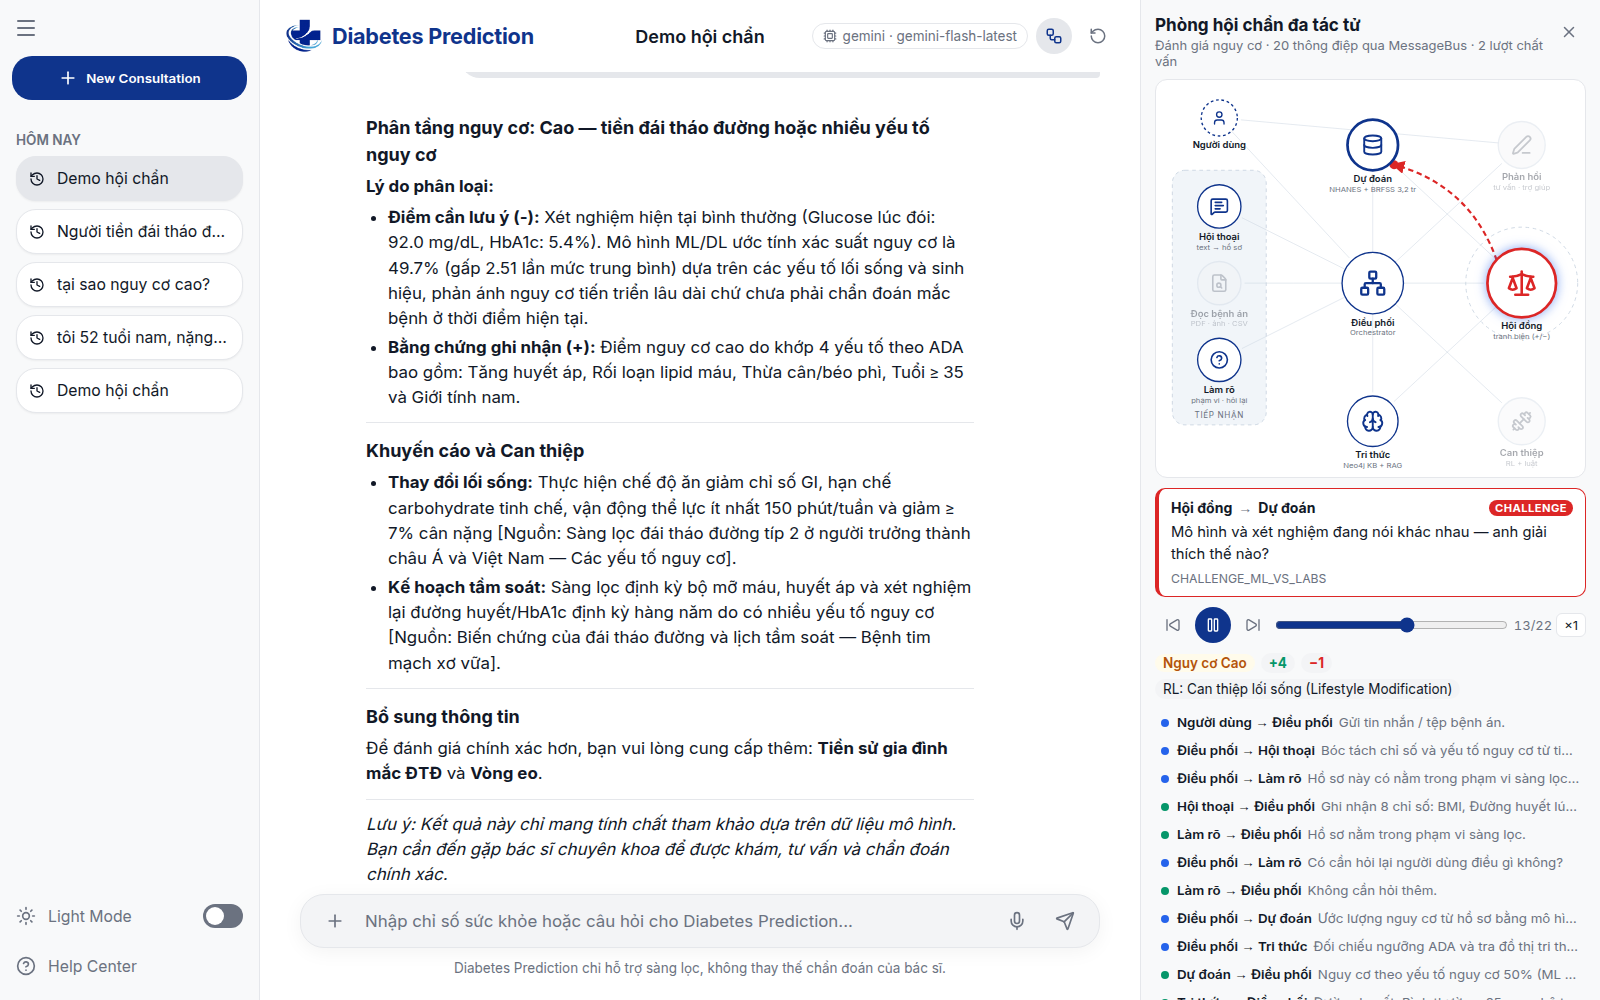
\includegraphics[width=\linewidth]{ui_debate.png}
\caption{Giao diện chatbot và Phòng hội chẩn: hội đồng đang chất vấn agent Dự đoán (mũi tên đỏ)}
\label{fig:ui-full}
\end{figure}

\begin{figure}[H]
\centering
\begin{minipage}[t]{0.32\linewidth}\centering
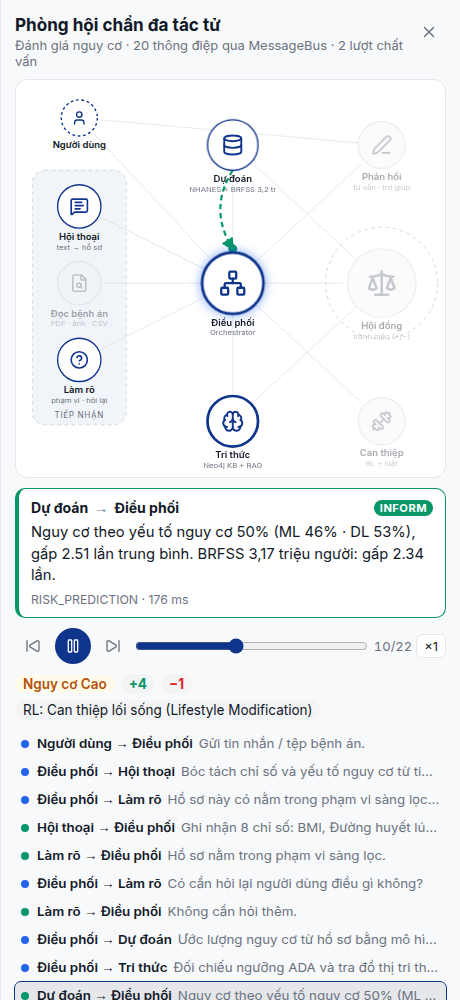
\includegraphics[width=\linewidth,trim=0 380 0 0,clip]{ui_branches_room.png}\\[-2pt]{\footnotesize (a) Nhánh DL trả kết quả}
\end{minipage}\hfill
\begin{minipage}[t]{0.32\linewidth}\centering
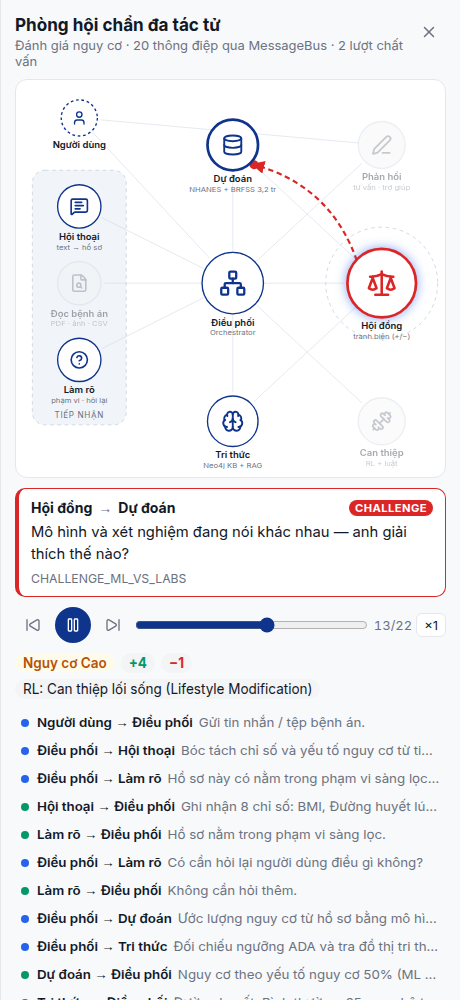
\includegraphics[width=\linewidth,trim=0 380 0 0,clip]{ui_debate_room.png}\\[-2pt]{\footnotesize (b) Hội đồng chất vấn}
\end{minipage}\hfill
\begin{minipage}[t]{0.32\linewidth}\centering
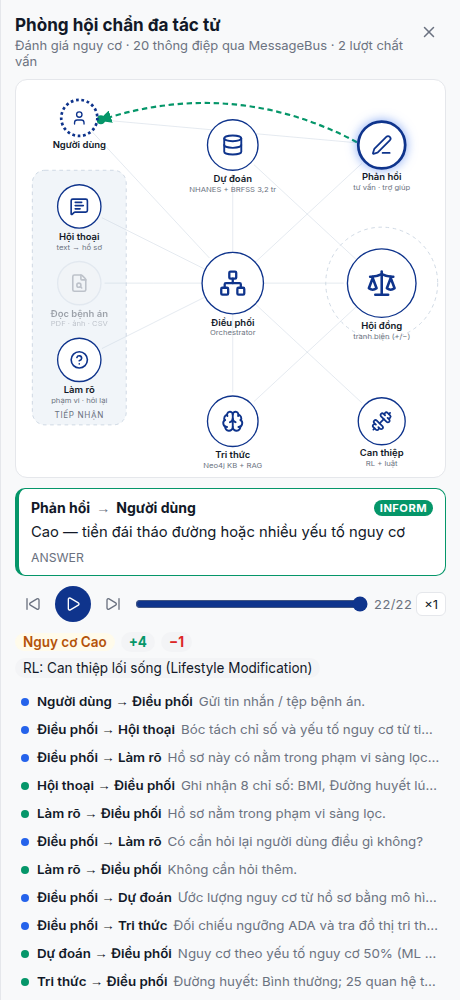
\includegraphics[width=\linewidth,trim=0 380 0 0,clip]{ui_final_room.png}\\[-2pt]{\footnotesize (c) Trả lời người dùng}
\end{minipage}
\caption{Ba thời điểm khi phát lại một lượt hội chẩn trong Phòng hội chẩn}
\label{fig:ui-steps}
\end{figure}

\subsection*{Khối ``Hội đồng đang suy luận'' trong khung chat}

Ngoài Phòng hội chẩn, phần suy luận còn hiện \emph{ngay trong khung chat} theo thời gian thực, giống cách các trợ lý AI hiển thị quá trình suy nghĩ. Endpoint \api{POST /api/chat/stream} trả về luồng NDJSON: \texttt{MessageBus} đẩy mỗi thông điệp ra ngay khi ghi nhận (qua một \texttt{ContextVar} gắn với lượt chat, nên các nhánh chạy song song bằng \texttt{asyncio.gather} cũng được đẩy ra). Khi agent Tri thức duyệt Neo4j, backend gửi thêm một sự kiện \texttt{graph} chứa đúng các nút và cạnh vừa đi qua, và giao diện vẽ ngay đồ thị đó: nút xuất phát ở giữa, nút cách 1 bước ở vòng trong, 2 bước ở vòng ngoài, tô màu theo nhãn ontology (\figref{fig:ui-thinking}a). Suy luận xong, khối tự thu gọn thành một dòng tóm tắt; người dùng bấm vào mới mở lại các bước và đồ thị (\figref{fig:ui-thinking}b).

\begin{figure}[H]
\centering
\begin{minipage}[t]{0.5\linewidth}\centering
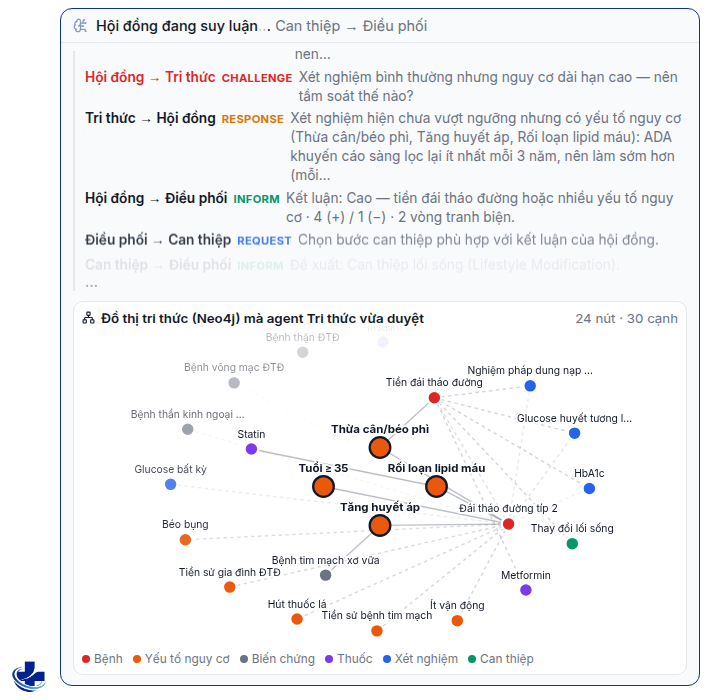
\includegraphics[width=\linewidth]{ui_thinking_live.png}\\[-2pt]{\footnotesize (a) Đang suy luận: từng thông điệp và đồ thị Neo4j vừa duyệt}
\end{minipage}\hfill
\begin{minipage}[t]{0.47\linewidth}\centering
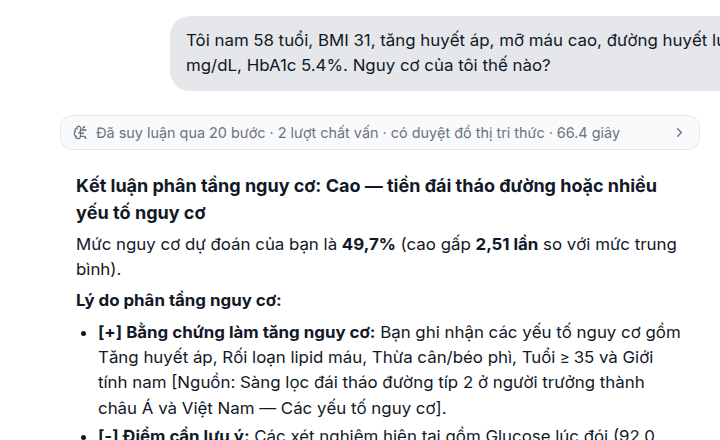
\includegraphics[width=\linewidth]{ui_thinking_done.png}\\[-2pt]{\footnotesize (b) Xong: thu gọn thành dropdown phía trên câu trả lời}
\end{minipage}
\caption{Khối suy luận của hội đồng trong khung chat}
\label{fig:ui-thinking}
\end{figure}

\section{Ví dụ một lượt hội chẩn}

Tin nhắn demo: ``Tôi nam 58 tuổi, BMI 31, tăng huyết áp, mỡ máu cao, đường huyết lúc đói 92 mg/dL, HbA1c 5.4\%. Nguy cơ của tôi thế nào?''. Đây là ca điển hình gây mâu thuẫn: xét nghiệm \emph{bình thường} nhưng yếu tố nguy cơ \emph{dày đặc}. Hệ thống chạy ở chế độ không LLM. \tabref{tab:transcript} là toàn bộ 22 thông điệp mà MessageBus ghi lại, kèm câu tóm tắt hiển thị trong Phòng hội chẩn.

\begin{table}[H]
\centering
\caption{Luồng 22 thông điệp của lượt hội chẩn demo (ms: thời gian xử lý ở thông điệp trả lời)}
\label{tab:transcript}
\scriptsize
\begin{tabularx}{\linewidth}{@{}r L{2.0cm} L{2.0cm} L{1.5cm} Y r@{}}
\toprule
\textbf{\#} & \textbf{Gửi} & \textbf{Nhận} & \textbf{Perf.} & \textbf{Nội dung (tóm tắt)} & \textbf{ms} \\
\midrule
1–2 & Orchestrator $\rightleftarrows$ & Conversation & REQ / INF & Ghi nhận 6 chỉ số: FPG, HbA1c, BMI, tuổi, tăng huyết áp, rối loạn mỡ máu & 3 \\
3–6 & Orchestrator $\rightleftarrows$ & Clarification & REQ / INF & Hồ sơ nằm trong phạm vi sàng lọc; không cần hỏi thêm & 0 \\
7, 9 & Orchestrator $\rightleftarrows$ & Prediction & REQ / INF & NHANES: nguy cơ 47\% (ML 45\% · DL 50\%), gấp 2,38 lần trung bình; BRFSS 3,17 triệu người: gấp 2,43 lần & 232 \\
8, 10 & Orchestrator $\rightleftarrows$ & Knowledge & REQ / INF & Đường huyết bình thường; 25 quan hệ trên đồ thị tri thức & 1.260 \\
11 & Orchestrator & Critic & REQUEST & Mở hội đồng: tổng hợp bằng chứng và tranh biện & \\
12 & Critic & Prediction & \textbf{CHALLENGE} & Hồ sơ còn thiếu nhiều đặc trưng — dự đoán còn tin được không? & \\
13 & Prediction & Critic & RESPONSE & Mới có 31\% đặc trưng; mô hình được huấn luyện cho dữ liệu thiếu, hạ độ tin cậy & 0 \\
14 & Critic & Prediction & \textbf{CHALLENGE} & Mô hình và xét nghiệm nói khác nhau — giải thích thế nào? & \\
15 & Prediction & Critic & RESPONSE & Mô hình không dùng glucose nên phản ánh nguy cơ tiến triển; đồng ý xét nghiệm là căn cứ chẩn đoán, đề nghị giữ tầm soát & 0 \\
16 & Critic & Knowledge & \textbf{CHALLENGE} & (vòng 2) Xét nghiệm bình thường nhưng nguy cơ dài hạn cao — tầm soát thế nào? & \\
17 & Knowledge & Critic & RESPONSE & ADA: sàng lọc lại ít nhất mỗi 3 năm, sớm hơn khi nhiều yếu tố nguy cơ; giảm cân, vận động 150 phút/tuần & 22 \\
18 & Critic & Orchestrator & INFORM & Kết luận: Cao — 5 (+) / 2 (−), 2 vòng tranh biện; có (+) ``mô hình quy mô lớn đồng thuận'' & 23 \\
19–20 & Orchestrator $\rightleftarrows$ & TreatmentRL & REQ / INF & Đề xuất: can thiệp lối sống (luật giới hạn vì xét nghiệm chưa ở ngưỡng ĐTĐ) & 0 \\
21–22 & Orchestrator $\rightleftarrows$ & Response & REQ / INF & Viết câu trả lời có trích dẫn & 0 \\
\bottomrule
\end{tabularx}
\end{table}

Ví dụ này cho thấy giá trị của tranh biện. Một hệ thống chỉ dùng ngưỡng sẽ trả lời ``đường huyết bình thường''. Một hệ thống chỉ dùng mô hình sẽ trả lời ``nguy cơ 47\%'' mà không giải thích vì sao xét nghiệm lại bình thường. Hội đồng đưa cả hai góc nhìn ra, hòa giải chúng thành một kế hoạch tầm soát có trích dẫn, và cho người dùng thấy cả điểm đồng thuận lẫn điểm còn cần lưu ý (hồ sơ còn thiếu giới tính, vòng eo, huyết áp, tiền sử gia đình). Hai mô hình huấn luyện trên hai quần thể khác nhau (20 nghìn người có xét nghiệm và 3,17 triệu người tự khai) cho nguy cơ tương đối gần như trùng nhau (2,38 và 2,43 lần), nên hội đồng ghi thêm một bằng chứng (+) độc lập. Toàn bộ phần ``suy nghĩ'' của hội đồng mất khoảng 1,3 giây, phần lớn là nhánh Tri thức trong lần gọi đầu (nạp mô hình nhúng và duyệt đồ thị).

\section{Kiểm thử}

\begin{table}[H]
\centering
\caption{Bộ kiểm thử tự động (43 kiểm thử, đều đạt)}
\label{tab:tests}
\small
\begin{tabularx}{\linewidth}{@{}L{4.4cm}Y@{}}
\toprule
\textbf{Tệp} & \textbf{Nội dung} \\
\midrule
\texttt{test\_clinical\_criteria.py} & Ngưỡng ADA cho FPG, HbA1c, OGTT; quy tắc ``2 kết quả bất thường'' \\
\texttt{test\_extraction.py} & Trích chỉ số từ tin nhắn tiếng Việt, quy đổi đơn vị, đọc PDF, ảnh, DOCX, CSV \\
\texttt{test\_scope.py} & Phát hiện hồ sơ ngoài phạm vi và kế hoạch câu hỏi làm rõ \\
\texttt{test\_large\_scale.py} & Hội đồng chỉ chất vấn khi mô hình NHANES và BRFSS nằm ở hai phía ngược nhau; phản hồi hạ độ tin cậy \\
\texttt{test\_summary.py} & Câu tóm tắt cho từng loại thông điệp trong Phòng hội chẩn \\
\texttt{test\_multi\_agent.py} & Cả hội đồng chạy trên SQLite + Qdrant + Neo4j: hỏi lại khi thiếu dữ liệu, tranh biện 2 vòng, câu hỏi kiến thức không chạy nhánh dự đoán, guardrail ghi đè, câu hỏi tiếp nối trả lời từ bộ nhớ \\
\bottomrule
\end{tabularx}
\end{table}

\section{Đánh giá đầu–cuối}

Hệ thống được đánh giá trên \textbf{400 ca} lấy ngẫu nhiên từ tập kiểm tra NHANES (\agent{PredictionAgent} chưa từng thấy), chỉ giữ người có cả FPG và HbA1c: 23,0\% mắc ĐTĐ. Đánh giá chạy không LLM để kết quả tất định, trên đúng bộ lưu trữ SQLite + Qdrant + Neo4j của project.

\begin{table}[H]
\centering
\caption{Đủ xét nghiệm (FPG + HbA1c): tính đúng đắn và vận hành của hội đồng (399 ca)}
\label{tab:k1}
\small
\begin{tabularx}{\linewidth}{@{}L{5.6cm}Y@{}}
\toprule
\textbf{Chỉ số} & \textbf{Kết quả} \\
\midrule
Phân loại đường huyết đúng ngưỡng ADA & \textbf{399/399 (100\%)} \\
Áp đúng quy tắc ``2 xét nghiệm bất thường'' & \textbf{71/71 (100\%)} \\
Dữ liệu ngoài miền sinh lý & 1 ca BMI 74,8 bị từ chối, hệ thống hỏi lại thay vì dự đoán \\
Số vòng tranh biện & 0 vòng: 288 ca · 1 vòng: 100 · 2 vòng: 11 \\
Chất vấn được mở & xác minh tiêu chí 71 · ML–DL bất đồng 30 · ML thấp nhưng xét nghiệm ĐTĐ 13 · ML cao nhưng xét nghiệm bình thường 11 → lịch tầm soát 11 · \textbf{NHANES–BRFSS bất đồng 10} \\
Mô hình quy mô lớn (BRFSS) & cùng phía với mô hình chính ở 97,5\% ca; trung bình 4,6 điểm (+) mỗi ca (3,7 khi chưa có BRFSS) \\
Safety Guardrail & ưu tiên 77 ca · khám sớm 11 ca \\
Gợi ý can thiệp (RL sau ràng buộc) & lối sống 358 · metformin 5 · phối hợp tim–thận 25 · chuyên khoa 11 \\
Thông điệp mỗi lượt & 16–22 (trung bình 16,7); 146 cặp CHALLENGE/RESPONSE \\
Độ trễ một lượt (không LLM) & trung vị 136 ms, p95 192 ms; Prediction 129 ms (4 mô hình + giải thích) ‖ Knowledge 73 ms chạy song song \\
\bottomrule
\end{tabularx}
\end{table}

\figw[0.95\linewidth]{ch7_ops}{Thời gian xử lý của từng agent và tần suất các loại chất vấn}

\begin{table}[H]
\centering
\caption{Chỉ có FPG: giá trị của việc phối hợp nhiều agent (399 ca, 91 người ĐTĐ)}
\label{tab:k2}
\small
\begin{tabular}{@{}lccccr@{}}
\toprule
\textbf{Cách ra quyết định} & \textbf{Độ nhạy} & \textbf{Đặc hiệu} & \textbf{PPV} & \textbf{F1} & \textbf{Số ca dương} \\
\midrule
Agent Tri thức đơn lẻ: FPG ≥ 126 & 0,582 & \textbf{1,000} & \textbf{1,000} & \textbf{0,736} & 53 \\
Agent Tri thức đơn lẻ: FPG ≥ 100 & 0,879 & 0,520 & 0,351 & 0,502 & 228 \\
Agent Dự đoán đơn lẻ: ML ≥ 30\% & 0,659 & 0,841 & 0,551 & 0,600 & 109 \\
\textbf{Hội đồng: mức Cao hoặc Rất cao} & \textbf{0,945} & 0,458 & 0,340 & 0,500 & 253 \\
\bottomrule
\end{tabular}
\end{table}

\figw[0.95\linewidth]{ch7_k2}{Độ nhạy, đặc hiệu của các cách ra quyết định, và tỉ lệ ĐTĐ thật theo mức nguy cơ của hội đồng}

\textbf{Nhận xét.} Hai agent đơn lẻ bỏ sót những nhóm khác nhau. Ngưỡng FPG ≥ 126 chính xác tuyệt đối nhưng chỉ bắt được 58\% người ĐTĐ: 38 người ĐTĐ có FPG dưới 126 (đang điều trị tốt, hoặc chỉ có HbA1c vượt ngưỡng). Hội đồng kết hợp xét nghiệm với mô hình đạt \textbf{độ nhạy 0,945}, bắt thêm \textbf{33/38} ca mà FPG bỏ sót. Điểm nguy cơ của hội đồng có AUC 0,876, cao hơn FPG đơn lẻ (0,862) và mô hình đơn lẻ (0,855). Cái giá là độ đặc hiệu 0,46. Đây là đánh đổi có chủ đích của một công cụ \emph{sàng lọc}: mức Cao nghĩa là ``nên làm thêm HbA1c hoặc OGTT'', một xét nghiệm rẻ, trong khi bỏ sót người bệnh thì đắt hơn nhiều. Phân tầng có ý nghĩa rõ: mức Rất cao 100\% là ĐTĐ thật (53/53), mức Thấp chỉ 1,6\% (2/128).

Với tin nhắn tiếng Việt tự do sinh từ mẫu câu (399 tin), bộ trích xuất regex lấy đúng 100\% các trường, và 91\% tin nhắn cho cùng mức nguy cơ như khi nhập form. Phần còn lại khác mức vì tin nhắn ngẫu nhiên lược bớt thông tin (vòng eo, huyết áp, tiền sử), chứ không phải do trích sai.

\section{Hạn chế và hướng phát triển}

\begin{itemize}
  \item \textbf{Mô hình}: trên NHANES, MLP chỉ nhỉnh hơn hồi quy logistic; cả hai bộ dữ liệu là của Hoa Kỳ, chưa hiệu chỉnh cho người Việt. BRFSS bổ sung 14.249 người gốc Á ở tập kiểm tra (AUC 0,85) nhưng có nhãn tự khai, bỏ sót người mắc chưa được chẩn đoán, nên chỉ dùng làm ý kiến thứ hai.
  \item \textbf{RAG}: embedding MiniLM yếu với tiếng Việt chuyên ngành, làm tìm kiếm lai kém hơn toàn văn đơn lẻ trên bộ 60 câu. Hướng sửa: đổi sang E5 đa ngôn ngữ (hit@3 0,98 trong thí nghiệm của tiểu luận) hoặc gán trọng số cho RRF; mở rộng KB và bộ câu hỏi đánh giá.
  \item \textbf{RL}: môi trường và hàm thưởng tự đặt, chưa học từ dữ liệu điều trị thật. Hướng phát triển: mô phỏng đường huyết theo giờ để agent học kế hoạch ăn uống và vận động hằng ngày.
  \item \textbf{Trích xuất không LLM}: regex còn bỏ sót một số cách viết, ví dụ ``Tôi nam 58 tuổi'' chưa nhận ra giới tính trong ca demo. Khi có LLM, phần này do Gemini đảm nhận.
  \item \textbf{Đánh giá}: số liệu tin nhắn tự do là cận trên lạc quan, vì tin nhắn sinh từ mẫu câu mà regex được viết để hiểu.
\end{itemize}

\unnumberedchapter{KẾT LUẬN}

Project đã hiện thực hóa sơ đồ hệ đa agent cho bệnh tiểu đường của đề bài thành một hệ thống chạy được đầu–cuối. Dữ liệu có sẵn của CDC, tổng cộng \textbf{3,19 triệu người} (NHANES 20.646 người có xét nghiệm và BRFSS 2011–2023 gồm 3.172.819 người), đi qua Deep Learning (\agent{PredictionAgent}: GBDT + MLP, AUC 0,83 trên cả hai bộ) để dự đoán và phân loại nguy cơ. Mô hình quy mô lớn làm ý kiến thứ hai và đồng thuận với mô hình chính ở 97,5\% ca. Tri thức từ hướng dẫn ADA 2024 và QĐ 5481/QĐ-BYT được tạo thành Knowledge Base gồm đồ thị 34 nút, 40 cạnh trên \textbf{Neo4j} và 36 đoạn văn được tìm kiếm lai trên \textbf{Qdrant} và \textbf{SQLite FTS5} (\agent{KnowledgeAgent}, hit@3 0,90). Reinforcement learning kết hợp luật (\agent{TreatmentRLAgent}) chọn bước can thiệp trong khuôn khổ an toàn. Các nhánh hội tụ ở một hội đồng tranh biện, nơi agent phản biện chất vấn agent chuyên môn khi chúng mâu thuẫn, rồi tư vấn và trợ giúp người dùng bằng câu trả lời có trích dẫn.

Đánh giá trên 400 ca NHANES chưa từng thấy cho thấy: lớp luật lâm sàng đúng tuyệt đối; phối hợp agent Tri thức với agent Dự đoán nâng độ nhạy phát hiện ĐTĐ từ 0,58 lên 0,95, với phân tầng có ý nghĩa (mức Rất cao 100\% là ĐTĐ, mức Thấp 1,6\%); tranh biện chỉ kích hoạt khi cần (26\% ca); một lượt hội chẩn đầy đủ, chạy bốn mô hình dự đoán, mất khoảng 0,14 giây khi không dùng LLM. Giao diện Phòng hội chẩn giúp người xem thấy trực tiếp các agent trao đổi thông điệp, chất vấn và đi đến đồng thuận.

Bài học lớn nhất của project là trong bài toán y tế, giá trị của hệ đa agent không nằm ở việc có nhiều agent, mà ở chỗ các agent với dữ liệu và phương pháp khác nhau \emph{kiểm tra chéo} lẫn nhau, mọi quyết định đều truy vết được tới một mô hình đã đánh giá hoặc một quy tắc có trích dẫn, và agent học luôn được đặt dưới sự giám sát của tri thức tường minh. Hướng phát triển tiếp theo gồm: thay embedding đa ngôn ngữ mạnh hơn cho RAG, hiệu chỉnh mô hình trên dữ liệu người Việt, và xây dựng môi trường mô phỏng đường huyết để agent RL học kế hoạch sinh hoạt hằng ngày.


\clearpage
\phantomsection
\addcontentsline{toc}{chapter}{TÀI LIỆU THAM KHẢO}
\begin{spacing}{1.1}
\begin{english}\printbibliography[title={TÀI LIỆU THAM KHẢO}]\end{english}
\end{spacing}

\end{document}
